% Options for packages loaded elsewhere
\PassOptionsToPackage{unicode}{hyperref}
\PassOptionsToPackage{hyphens}{url}
%
\documentclass[
]{article}
\usepackage{amsmath,amssymb}
\usepackage{iftex}
\ifPDFTeX
  \usepackage[T1]{fontenc}
  \usepackage[utf8]{inputenc}
  \usepackage{textcomp} % provide euro and other symbols
\else % if luatex or xetex
  \usepackage{unicode-math} % this also loads fontspec
  \defaultfontfeatures{Scale=MatchLowercase}
  \defaultfontfeatures[\rmfamily]{Ligatures=TeX,Scale=1}
\fi
\usepackage{lmodern}
\ifPDFTeX\else
  % xetex/luatex font selection
\fi
% Use upquote if available, for straight quotes in verbatim environments
\IfFileExists{upquote.sty}{\usepackage{upquote}}{}
\IfFileExists{microtype.sty}{% use microtype if available
  \usepackage[]{microtype}
  \UseMicrotypeSet[protrusion]{basicmath} % disable protrusion for tt fonts
}{}
\makeatletter
\@ifundefined{KOMAClassName}{% if non-KOMA class
  \IfFileExists{parskip.sty}{%
    \usepackage{parskip}
  }{% else
    \setlength{\parindent}{0pt}
    \setlength{\parskip}{6pt plus 2pt minus 1pt}}
}{% if KOMA class
  \KOMAoptions{parskip=half}}
\makeatother
\usepackage{xcolor}
\usepackage[margin=1in]{geometry}
\usepackage{color}
\usepackage{fancyvrb}
\newcommand{\VerbBar}{|}
\newcommand{\VERB}{\Verb[commandchars=\\\{\}]}
\DefineVerbatimEnvironment{Highlighting}{Verbatim}{commandchars=\\\{\}}
% Add ',fontsize=\small' for more characters per line
\usepackage{framed}
\definecolor{shadecolor}{RGB}{248,248,248}
\newenvironment{Shaded}{\begin{snugshade}}{\end{snugshade}}
\newcommand{\AlertTok}[1]{\textcolor[rgb]{0.94,0.16,0.16}{#1}}
\newcommand{\AnnotationTok}[1]{\textcolor[rgb]{0.56,0.35,0.01}{\textbf{\textit{#1}}}}
\newcommand{\AttributeTok}[1]{\textcolor[rgb]{0.13,0.29,0.53}{#1}}
\newcommand{\BaseNTok}[1]{\textcolor[rgb]{0.00,0.00,0.81}{#1}}
\newcommand{\BuiltInTok}[1]{#1}
\newcommand{\CharTok}[1]{\textcolor[rgb]{0.31,0.60,0.02}{#1}}
\newcommand{\CommentTok}[1]{\textcolor[rgb]{0.56,0.35,0.01}{\textit{#1}}}
\newcommand{\CommentVarTok}[1]{\textcolor[rgb]{0.56,0.35,0.01}{\textbf{\textit{#1}}}}
\newcommand{\ConstantTok}[1]{\textcolor[rgb]{0.56,0.35,0.01}{#1}}
\newcommand{\ControlFlowTok}[1]{\textcolor[rgb]{0.13,0.29,0.53}{\textbf{#1}}}
\newcommand{\DataTypeTok}[1]{\textcolor[rgb]{0.13,0.29,0.53}{#1}}
\newcommand{\DecValTok}[1]{\textcolor[rgb]{0.00,0.00,0.81}{#1}}
\newcommand{\DocumentationTok}[1]{\textcolor[rgb]{0.56,0.35,0.01}{\textbf{\textit{#1}}}}
\newcommand{\ErrorTok}[1]{\textcolor[rgb]{0.64,0.00,0.00}{\textbf{#1}}}
\newcommand{\ExtensionTok}[1]{#1}
\newcommand{\FloatTok}[1]{\textcolor[rgb]{0.00,0.00,0.81}{#1}}
\newcommand{\FunctionTok}[1]{\textcolor[rgb]{0.13,0.29,0.53}{\textbf{#1}}}
\newcommand{\ImportTok}[1]{#1}
\newcommand{\InformationTok}[1]{\textcolor[rgb]{0.56,0.35,0.01}{\textbf{\textit{#1}}}}
\newcommand{\KeywordTok}[1]{\textcolor[rgb]{0.13,0.29,0.53}{\textbf{#1}}}
\newcommand{\NormalTok}[1]{#1}
\newcommand{\OperatorTok}[1]{\textcolor[rgb]{0.81,0.36,0.00}{\textbf{#1}}}
\newcommand{\OtherTok}[1]{\textcolor[rgb]{0.56,0.35,0.01}{#1}}
\newcommand{\PreprocessorTok}[1]{\textcolor[rgb]{0.56,0.35,0.01}{\textit{#1}}}
\newcommand{\RegionMarkerTok}[1]{#1}
\newcommand{\SpecialCharTok}[1]{\textcolor[rgb]{0.81,0.36,0.00}{\textbf{#1}}}
\newcommand{\SpecialStringTok}[1]{\textcolor[rgb]{0.31,0.60,0.02}{#1}}
\newcommand{\StringTok}[1]{\textcolor[rgb]{0.31,0.60,0.02}{#1}}
\newcommand{\VariableTok}[1]{\textcolor[rgb]{0.00,0.00,0.00}{#1}}
\newcommand{\VerbatimStringTok}[1]{\textcolor[rgb]{0.31,0.60,0.02}{#1}}
\newcommand{\WarningTok}[1]{\textcolor[rgb]{0.56,0.35,0.01}{\textbf{\textit{#1}}}}
\usepackage{graphicx}
\makeatletter
\def\maxwidth{\ifdim\Gin@nat@width>\linewidth\linewidth\else\Gin@nat@width\fi}
\def\maxheight{\ifdim\Gin@nat@height>\textheight\textheight\else\Gin@nat@height\fi}
\makeatother
% Scale images if necessary, so that they will not overflow the page
% margins by default, and it is still possible to overwrite the defaults
% using explicit options in \includegraphics[width, height, ...]{}
\setkeys{Gin}{width=\maxwidth,height=\maxheight,keepaspectratio}
% Set default figure placement to htbp
\makeatletter
\def\fps@figure{htbp}
\makeatother
\setlength{\emergencystretch}{3em} % prevent overfull lines
\providecommand{\tightlist}{%
  \setlength{\itemsep}{0pt}\setlength{\parskip}{0pt}}
\setcounter{secnumdepth}{-\maxdimen} % remove section numbering
\ifLuaTeX
  \usepackage{selnolig}  % disable illegal ligatures
\fi
\IfFileExists{bookmark.sty}{\usepackage{bookmark}}{\usepackage{hyperref}}
\IfFileExists{xurl.sty}{\usepackage{xurl}}{} % add URL line breaks if available
\urlstyle{same}
\hypersetup{
  pdftitle={Seminario Fuentes de datos Biómédicas y Web Semántica},
  pdfauthor={Urko Alli Barrena, Paula Gregorio Losada, Victoria Garcia Lovelle},
  hidelinks,
  pdfcreator={LaTeX via pandoc}}

\title{Seminario Fuentes de datos Biómédicas y Web Semántica}
\usepackage{etoolbox}
\makeatletter
\providecommand{\subtitle}[1]{% add subtitle to \maketitle
  \apptocmd{\@title}{\par {\large #1 \par}}{}{}
}
\makeatother
\subtitle{Relación entre la Esperanza de Vida y el consumo de Agua}
\author{Urko Alli Barrena, Paula Gregorio Losada, Victoria Garcia
Lovelle}
\date{2023-12-10}

\begin{document}
\maketitle

{
\setcounter{tocdepth}{6}
\tableofcontents
}

\includegraphics[width=2.60417in,height=0.9375in]{INPUT/images/EscudoUBU.png}

\hypertarget{introducciuxf3n}{%
\section{1. Introducción}\label{introducciuxf3n}}

En el desarrollo de este seminario, analizaremos cómo diversos aspectos
relacionados con la calidad y cantidad de agua consumida pueden influir
en la esperanza de vida en las diferentes Comunidades Autónomas de
España.

Exploraremos detalladamente cómo la calidad del agua, medida a través de
diferentes parámetros, y la cantidad de agua, pueden ser factores
determinantes para la salud y, consecuentemente, para la esperanza de
vida de las Comunidades Autónomas.

\hypertarget{objetivos}{%
\section{2. Objetivos}\label{objetivos}}

El objetivo principal de este seminario es analizar de manera formal
cómo diversos aspectos relacionados con la calidad y la cantidad de agua
consumida pueden afectar en la esperanza de vida en las distintas
Comunidades Autónomas de España. Se explorarán los siguientes puntos:

\begin{enumerate}
\def\labelenumi{\arabic{enumi}.}
\item
  \textbf{Observar si la calidad del agua afecta directamente en la
  esperanza de vida}: Investigar cómo la calidad del agua puede tener
  repercusiones directas en la esperanza de vida de la población
  española por Comunidades Autónomas.
\item
  \textbf{Observar si la cantidad de agua consumida afecta directamente
  en la esperanza de vida}: Analizar de manera detallada cómo la
  cantidad de agua consumida puede influir en la esperanza de vida de la
  población española por Comunidades Autónomas.
\item
  \textbf{Observar si afecta el presupuesto para potabilizar el agua con
  la cantidad de agua consumida}: Evaluar la relación entre el
  presupuesto destinado a la potabilización del agua y la cantidad de
  agua consumida, explorando posibles implicaciones para la esperanza de
  vida.
\item
  \textbf{Impacto combinado de la calidad y cantidad de agua en la
  Esperanza de Vida}: Estudiar cómo la interacción entre la calidad y la
  cantidad de agua consumida puede tener un impacto significativo en la
  esperanza de vida de la población española por Comunidades Autónomas.
\end{enumerate}

\hypertarget{carga-de-libreruxedas}{%
\section{3. Carga de librerías}\label{carga-de-libreruxedas}}

\begin{enumerate}
\def\labelenumi{\arabic{enumi}.}
\tightlist
\item
  \emph{pdftools:} Esta librería se utilizó para extraer datos de
  archivos PDF. En particular, se empleó para obtener información
  relevante sobre la calidad del agua de un informe en formato PDF.
\end{enumerate}

\begin{Shaded}
\begin{Highlighting}[]
\FunctionTok{library}\NormalTok{(pdftools)}
\end{Highlighting}
\end{Shaded}

\begin{enumerate}
\def\labelenumi{\arabic{enumi}.}
\setcounter{enumi}{1}
\tightlist
\item
  \emph{tidyverse}: Un conjunto de paquetes que facilitan la
  manipulación y visualización de datos en R. Incluye librerías como
  tidyr y dplyr, las cuales fueron esenciales para organizar y
  transformar datos.
\end{enumerate}

\begin{Shaded}
\begin{Highlighting}[]
\FunctionTok{library}\NormalTok{(tidyverse)}
\end{Highlighting}
\end{Shaded}

\begin{enumerate}
\def\labelenumi{\arabic{enumi}.}
\setcounter{enumi}{2}
\tightlist
\item
  \emph{tidyjson}: Esta librería fue útil para trabajar con datos en
  formato JSON. Fue esencial para analizar y extraer información de
  archivos JSON relacionados con la esperanza de vida y la cantidad de
  agua.
\end{enumerate}

\begin{Shaded}
\begin{Highlighting}[]
\FunctionTok{library}\NormalTok{(tidyjson)}
\end{Highlighting}
\end{Shaded}

\begin{enumerate}
\def\labelenumi{\arabic{enumi}.}
\setcounter{enumi}{3}
\tightlist
\item
  \emph{rjson}: Se utilizó para cargar y procesar datos almacenados en
  formato JSON. Facilita la manipulación de datos estructurados y su
  conversión a formatos compatibles con R.
\end{enumerate}

\begin{Shaded}
\begin{Highlighting}[]
\FunctionTok{library}\NormalTok{(rjson) }
\end{Highlighting}
\end{Shaded}

\hypertarget{obtenciuxf3n-de-tablas}{%
\section{4. Obtención de tablas}\label{obtenciuxf3n-de-tablas}}

\hypertarget{tabla-de-esperanza-de-vida}{%
\subsubsection{4.1. Tabla de Esperanza de
Vida}\label{tabla-de-esperanza-de-vida}}

Para obtener la tabla de esperanza de vida se cargan los datos desde un
archivo \emph{Json}.

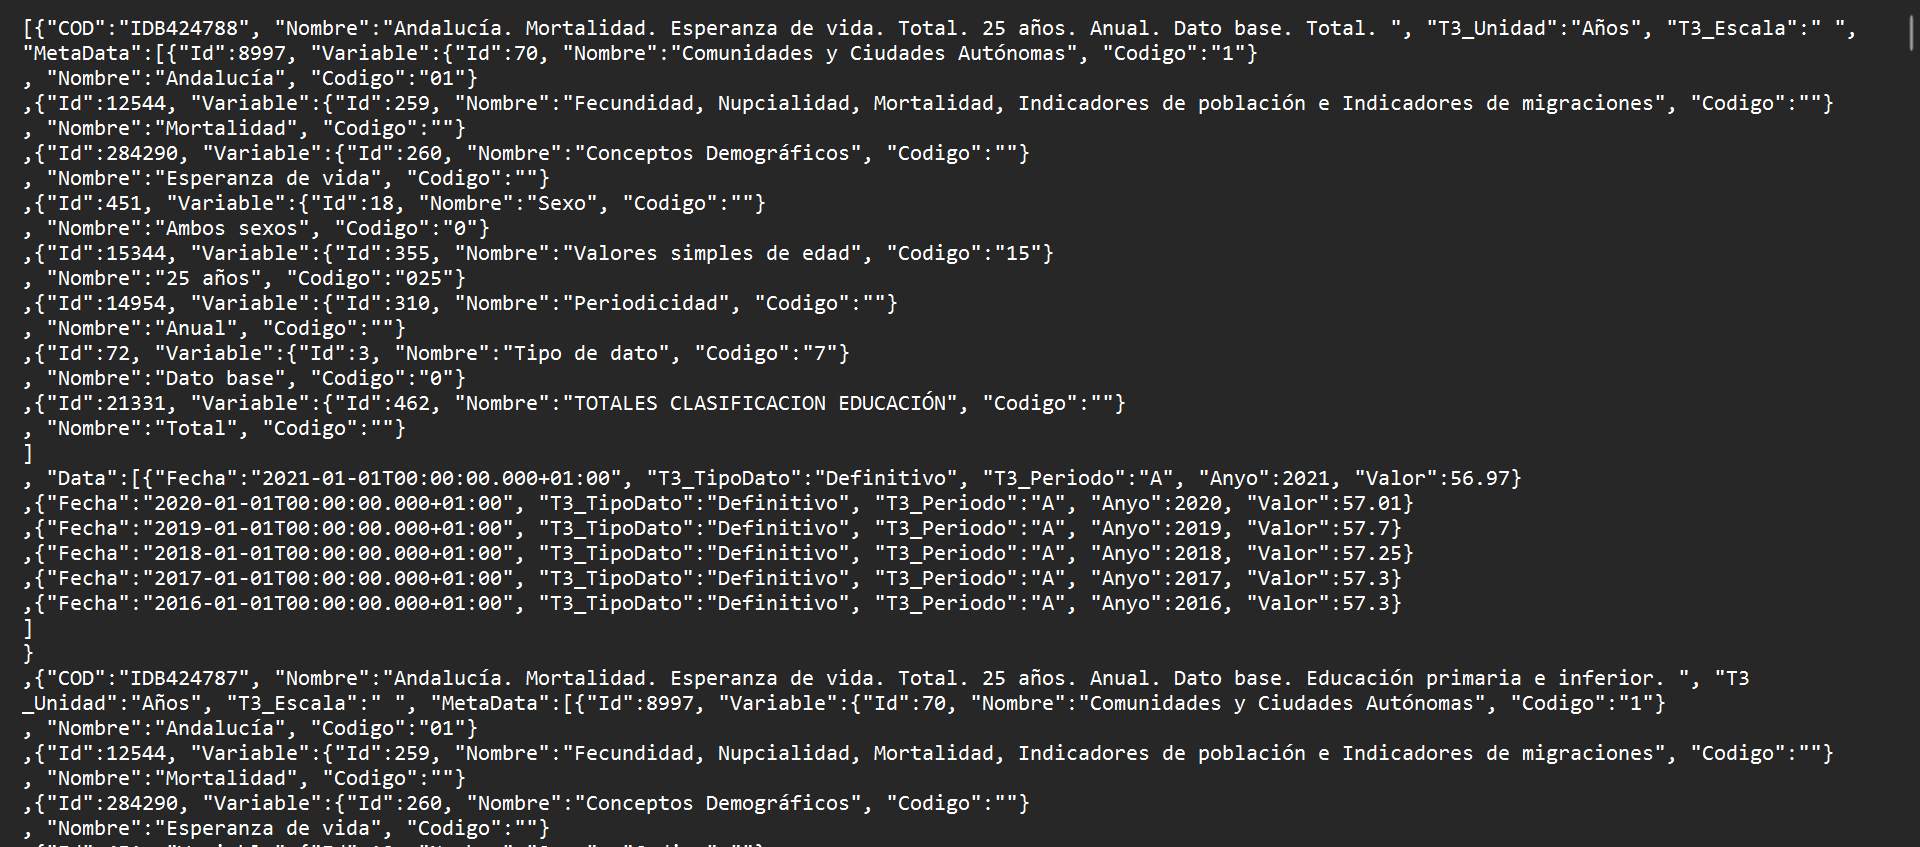
\includegraphics{INPUT/images/EsperanzadeVidaJson.png}

Esto es una porción de todo el archivo \emph{Json}, del cual se tiene
que seleccionar los datos deseados.

Una vez cargados los datos, se organizan en un formato de tabla y se
realiza un análisis para saber qué tipos contiene la variable
``EsperanzaVida''.

\begin{Shaded}
\begin{Highlighting}[]
\NormalTok{archivoJson }\OtherTok{\textless{}{-}} \FunctionTok{fromJSON}\NormalTok{(}\AttributeTok{file =} \StringTok{"INPUT/data/EsperanzaVida.json"}\NormalTok{)}

\NormalTok{esperanzaVida }\OtherTok{\textless{}{-}} \FunctionTok{spread\_all}\NormalTok{(archivoJson)}

\NormalTok{tibble1}\OtherTok{\textless{}{-}}\NormalTok{esperanzaVida }\SpecialCharTok{\%\textgreater{}\%} 
\NormalTok{  gather\_object }\SpecialCharTok{\%\textgreater{}\%}  
\NormalTok{  json\_types }\SpecialCharTok{\%\textgreater{}\%} 
  \FunctionTok{count}\NormalTok{(name, type)}
\end{Highlighting}
\end{Shaded}

Para obtener la tabla final se ha accedido a aquel que era de tipo
\emph{array} que contiene los valores de interés y organiza estos datos
en una tabla.

\begin{Shaded}
\begin{Highlighting}[]
\NormalTok{arrayData}\OtherTok{\textless{}{-}}\NormalTok{esperanzaVida }\SpecialCharTok{\%\textgreater{}\%}
  \FunctionTok{enter\_object}\NormalTok{(Data) }\SpecialCharTok{\%\textgreater{}\%} 
\NormalTok{  gather\_array }\SpecialCharTok{\%\textgreater{}\%} 
\NormalTok{  spread\_all }\SpecialCharTok{\%\textgreater{}\%} 
  \FunctionTok{select}\NormalTok{(Nombre, Anyo, Valor) }
\end{Highlighting}
\end{Shaded}

El atributo ``Nombre'' contiene una cadena de caracteres muy larga
separada por puntos. Entre toda la información estan los nombres de las
diferentes Comunidades Autónomas, por lo que se separa la cadena de
texto y se obtienen únicamente estos nombres.

\begin{Shaded}
\begin{Highlighting}[]
\NormalTok{partes }\OtherTok{\textless{}{-}} \FunctionTok{strsplit}\NormalTok{(arrayData}\SpecialCharTok{$}\NormalTok{Nombre, }\StringTok{"}\SpecialCharTok{\textbackslash{}\textbackslash{}}\StringTok{."}\NormalTok{)}

\NormalTok{comunidadesAutonomas}\OtherTok{\textless{}{-}}\FunctionTok{c}\NormalTok{()}
\ControlFlowTok{for}\NormalTok{ (i }\ControlFlowTok{in}\NormalTok{ partes)\{}
\NormalTok{  comunidadesAutonomas}\OtherTok{\textless{}{-}}\FunctionTok{c}\NormalTok{(comunidadesAutonomas,i[}\DecValTok{1}\NormalTok{])}
\NormalTok{\}}

\NormalTok{arrayData}\SpecialCharTok{$}\NormalTok{Nombre}\OtherTok{\textless{}{-}}\NormalTok{comunidadesAutonomas}
\end{Highlighting}
\end{Shaded}

De la tabla se obtiene el año 2020 de cada Comunidad Autónoma y se
obtiene como valor la media de la esperanza de vida en ese año.

Para tener todas las tablas con el mismo estilo, se han pasado los
nombres de las Comunidades Autónomas a mayúsculas.

\begin{Shaded}
\begin{Highlighting}[]
\NormalTok{tablaComunidadesAñoValor}\OtherTok{\textless{}{-}} \FunctionTok{as\_tibble}\NormalTok{(arrayData)}
\FunctionTok{attr}\NormalTok{(tablaComunidadesAñoValor, }\StringTok{"JSON"}\NormalTok{) }\OtherTok{\textless{}{-}} \ConstantTok{NULL}

\NormalTok{tablaEsperanzaDeVida }\OtherTok{\textless{}{-}}\NormalTok{ tablaComunidadesAñoValor }\SpecialCharTok{\%\textgreater{}\%}
  \FunctionTok{filter}\NormalTok{(Anyo}\SpecialCharTok{==}\DecValTok{2020}\NormalTok{)}\SpecialCharTok{\%\textgreater{}\%}
  \FunctionTok{group\_by}\NormalTok{(Anyo, Nombre) }\SpecialCharTok{\%\textgreater{}\%}
  \FunctionTok{summarize}\NormalTok{(}\AttributeTok{EsperanzaDeVida =} \FunctionTok{mean}\NormalTok{(Valor, }\AttributeTok{na.rm =} \ConstantTok{TRUE}\NormalTok{))}\SpecialCharTok{\%\textgreater{}\%}
  \FunctionTok{rename}\NormalTok{(Año}\OtherTok{=}\NormalTok{Anyo,}\AttributeTok{ComunidadAutonoma=}\NormalTok{Nombre)}

\NormalTok{tablaEsperanzaDeVidaFinal }\OtherTok{\textless{}{-}}\NormalTok{ tablaEsperanzaDeVida }\SpecialCharTok{\%\textgreater{}\%}
  \FunctionTok{mutate}\NormalTok{(}\AttributeTok{ComunidadAutonoma =} \FunctionTok{toupper}\NormalTok{(ComunidadAutonoma))}

\FunctionTok{colnames}\NormalTok{(tablaEsperanzaDeVidaFinal) }\OtherTok{\textless{}{-}} \FunctionTok{c}\NormalTok{(}\StringTok{"Anio"}\NormalTok{, }\StringTok{"ComunidadAutonoma"}\NormalTok{, }\StringTok{"EsperanzaDeVida"}\NormalTok{)}
\end{Highlighting}
\end{Shaded}

En la tabla final, se puede observar la media de la esperanza de vida de
cada Comunidad Autónoma en el año 2020.

\begin{Shaded}
\begin{Highlighting}[]
\NormalTok{tablaEsperanzaDeVidaFinal}
\end{Highlighting}
\end{Shaded}

\begin{verbatim}
## # A tibble: 19 x 3
## # Groups:   Anio [1]
##     Anio ComunidadAutonoma           EsperanzaDeVida
##    <dbl> <chr>                                 <dbl>
##  1  2020 ANDALUCÍA                              28.0
##  2  2020 ARAGÓN                                 28.4
##  3  2020 ASTURIAS, PRINCIPADO DE                28.1
##  4  2020 BALEARS, ILLES                         29.3
##  5  2020 CANARIAS                               29.1
##  6  2020 CANTABRIA                              28.9
##  7  2020 CASTILLA - LA MANCHA                   27.5
##  8  2020 CASTILLA Y LEÓN                        28.5
##  9  2020 CATALUÑA                               28.3
## 10  2020 CEUTA                                  26.7
## 11  2020 COMUNITAT VALENCIANA                   28.5
## 12  2020 EXTREMADURA                            27.9
## 13  2020 GALICIA                                29.3
## 14  2020 MADRID, COMUNIDAD DE                   28.0
## 15  2020 MELILLA                                26.3
## 16  2020 MURCIA, REGIÓN DE                      28.4
## 17  2020 NAVARRA, COMUNIDAD FORAL DE            29.0
## 18  2020 PAÍS VASCO                             28.8
## 19  2020 RIOJA, LA                              28.6
\end{verbatim}

\hypertarget{tabla-de-la-cantidad-de-agua}{%
\subsubsection{4.2. Tabla de la Cantidad de
Agua}\label{tabla-de-la-cantidad-de-agua}}

Para obtener la tabla de Cantidad de Agua se cargan los datos desde un
archivo \emph{Json}.

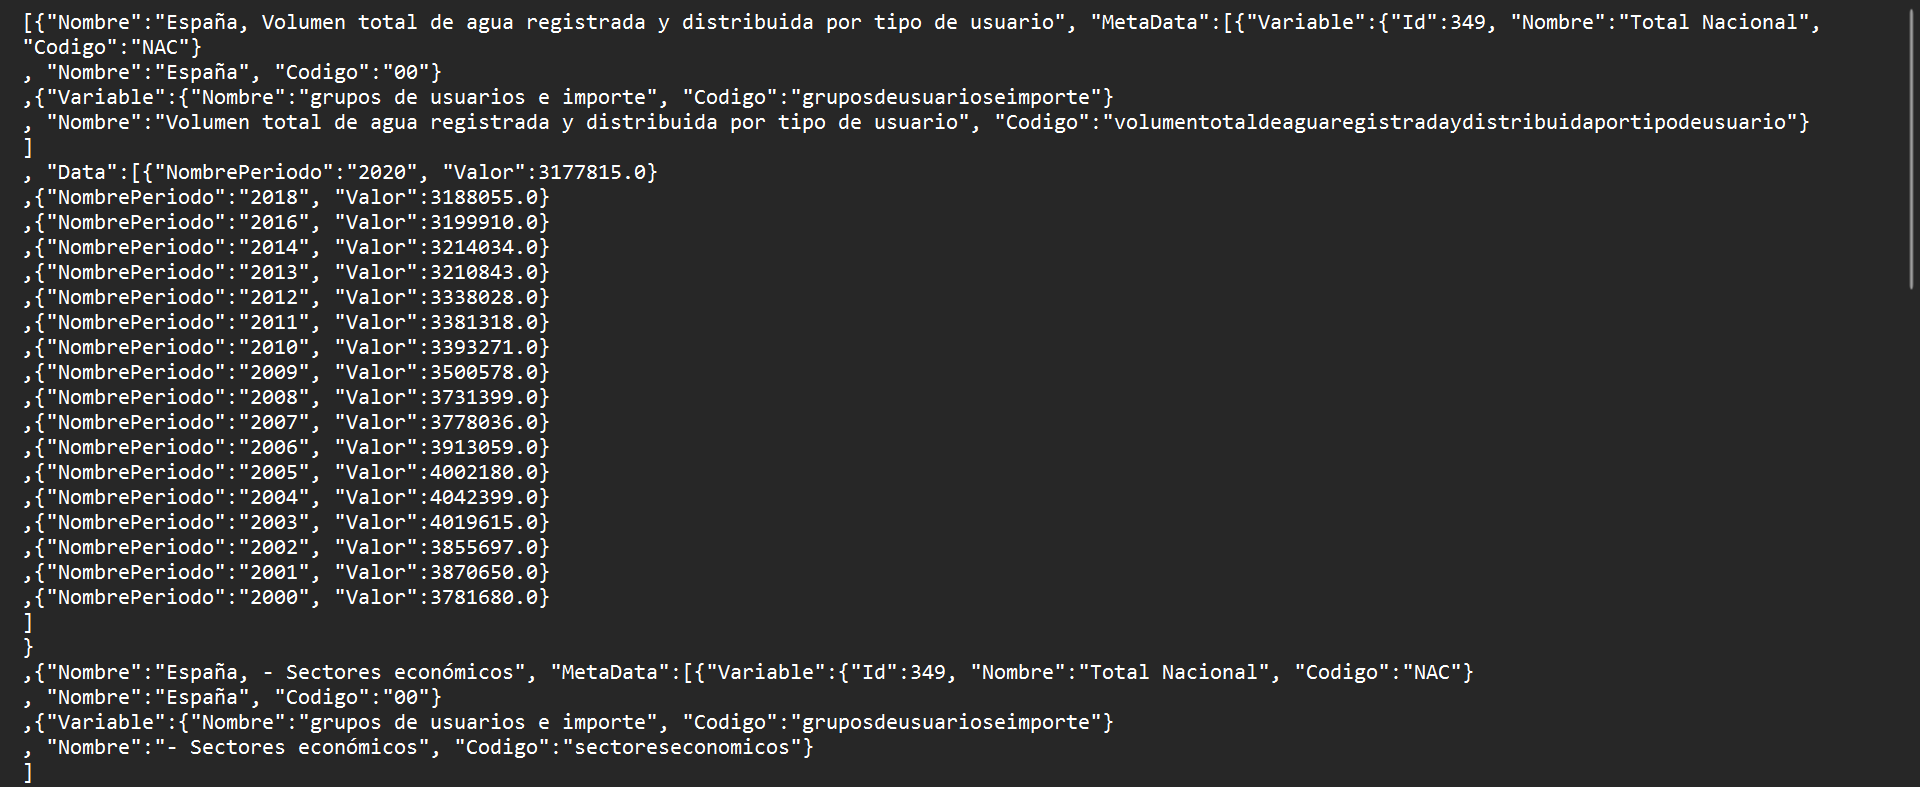
\includegraphics{INPUT/images/CantidadAguaJSON.png}

Esto es una porción de todo el archivo \emph{Json}, del cual se tiene
que seleccionar los datos deseados.

Una vez cargados los datos, se organizan en un formato de tabla y se
realiza un análisis para saber qué tipos contiene la variable
``cantidadAgua''.

\begin{Shaded}
\begin{Highlighting}[]
\NormalTok{archivoJsonCantidad }\OtherTok{\textless{}{-}} \FunctionTok{fromJSON}\NormalTok{(}\AttributeTok{file =} \StringTok{"INPUT/data/CantidadAgua.json"}\NormalTok{)}

\NormalTok{cantidadAgua }\OtherTok{\textless{}{-}} \FunctionTok{spread\_all}\NormalTok{(archivoJsonCantidad)}

\NormalTok{cantidadAgua}\SpecialCharTok{\%\textgreater{}\%}
\NormalTok{  gather\_object}\SpecialCharTok{\%\textgreater{}\%}
\NormalTok{  json\_types}\SpecialCharTok{\%\textgreater{}\%}
  \FunctionTok{count}\NormalTok{(name,type)}
\end{Highlighting}
\end{Shaded}

\begin{verbatim}
## # A tibble: 3 x 3
##   name     type       n
##   <chr>    <fct>  <int>
## 1 Data     array    133
## 2 MetaData array    133
## 3 Nombre   string   133
\end{verbatim}

Para poder obtener la tabla final de la cantidad de agua consumida en
cada Comunidad Autónoma, se ha accedido al atributo de tipo \emph{array}
que contiene la información de interés que es Data y organiza estos
datos en una tabla.

Seguidamente, como únicamente necesitamos las Comunidades Autónomas y
están escritas en una larga cadena de texto, dividimos la cadena de
texto y obtenemos de ella el nombre de las Comunidades Autónomas.

Esa nueva variable con las Comunidades Autónomas se añaden a la tabla
final y se elimina donde ponga España.

\begin{Shaded}
\begin{Highlighting}[]
\NormalTok{arrayDataCantidad}\OtherTok{\textless{}{-}}\NormalTok{cantidadAgua}\SpecialCharTok{\%\textgreater{}\%}
  \FunctionTok{enter\_object}\NormalTok{(Data)}\SpecialCharTok{\%\textgreater{}\%}
\NormalTok{  gather\_array}\SpecialCharTok{\%\textgreater{}\%}
\NormalTok{  spread\_all}\SpecialCharTok{\%\textgreater{}\%}
  \FunctionTok{select}\NormalTok{(}\SpecialCharTok{{-}}\NormalTok{document.id,}\SpecialCharTok{{-}}\NormalTok{array.index)}

\NormalTok{cadenas }\OtherTok{\textless{}{-}} \FunctionTok{strsplit}\NormalTok{(arrayDataCantidad}\SpecialCharTok{$}\NormalTok{Nombre, }\StringTok{"}\SpecialCharTok{\textbackslash{}\textbackslash{}}\StringTok{,"}\NormalTok{)}

\NormalTok{comunidadesAutonomasCantidad}\OtherTok{\textless{}{-}}\FunctionTok{c}\NormalTok{()}
\ControlFlowTok{for}\NormalTok{ (i }\ControlFlowTok{in}\NormalTok{ cadenas)\{}
\NormalTok{  comunidadesAutonomasCantidad}\OtherTok{\textless{}{-}}\FunctionTok{c}\NormalTok{(comunidadesAutonomasCantidad,i[}\DecValTok{1}\NormalTok{])}
\NormalTok{\}}

\NormalTok{arrayDataCantidad}\SpecialCharTok{$}\NormalTok{Nombre}\OtherTok{\textless{}{-}}\NormalTok{comunidadesAutonomasCantidad}

\NormalTok{tabla }\OtherTok{\textless{}{-}}\NormalTok{ arrayDataCantidad }\SpecialCharTok{\%\textgreater{}\%}
  \FunctionTok{filter}\NormalTok{(}\SpecialCharTok{!}\NormalTok{(Nombre }\SpecialCharTok{==} \StringTok{"España"}\NormalTok{)) }\SpecialCharTok{\%\textgreater{}\%}
  \FunctionTok{select}\NormalTok{(Nombre, NombrePeriodo, Valor)}
\end{Highlighting}
\end{Shaded}

Se filtra únicamente por el año 2020, que es el año de interés, se
realiza una media de los valores obtenidos en el año 2020 de cada
Comuniad Autónoma.

Para tener todas las tablas con el mismo estilo, se han pasado los
nombres de las Comunidades Autónomas a mayúsculas y se han renombrado.

Por último se ha pasado a tipo entero la columna años.

\begin{Shaded}
\begin{Highlighting}[]
\NormalTok{tablaCantidadDeAgua }\OtherTok{\textless{}{-}}\NormalTok{ tabla }\SpecialCharTok{\%\textgreater{}\%}
  \FunctionTok{filter}\NormalTok{(NombrePeriodo  }\SpecialCharTok{==}\DecValTok{2020}\NormalTok{)}\SpecialCharTok{\%\textgreater{}\%}
  \FunctionTok{group\_by}\NormalTok{(NombrePeriodo  , Nombre) }\SpecialCharTok{\%\textgreater{}\%}
  \FunctionTok{summarize}\NormalTok{(}\AttributeTok{Cantidad =} \FunctionTok{mean}\NormalTok{(Valor, }\AttributeTok{na.rm =} \ConstantTok{TRUE}\NormalTok{))}\SpecialCharTok{\%\textgreater{}\%}
  \FunctionTok{rename}\NormalTok{(Año}\OtherTok{=}\NormalTok{NombrePeriodo,}\AttributeTok{ComunidadAutonoma=}\NormalTok{Nombre)}

\NormalTok{tablaCantidadDeAgua }\OtherTok{\textless{}{-}}\NormalTok{ tablaCantidadDeAgua }\SpecialCharTok{\%\textgreater{}\%}
  \FunctionTok{mutate}\NormalTok{(}\AttributeTok{ComunidadAutonoma =} \FunctionTok{toupper}\NormalTok{(ComunidadAutonoma))}

\NormalTok{tablaCantidadDeAgua[}\DecValTok{4}\NormalTok{,}\DecValTok{2}\NormalTok{] }\OtherTok{\textless{}{-}} \FunctionTok{c}\NormalTok{(}\StringTok{"BALEARS, ILLES"}\NormalTok{)}
\NormalTok{tablaCantidadDeAgua[}\DecValTok{8}\NormalTok{,}\DecValTok{2}\NormalTok{] }\OtherTok{\textless{}{-}} \FunctionTok{c}\NormalTok{(}\StringTok{"CASTILLA {-} LA MANCHA"}\NormalTok{)}
\NormalTok{tablaCantidadDeAgua[}\DecValTok{14}\NormalTok{,}\DecValTok{2}\NormalTok{] }\OtherTok{\textless{}{-}} \FunctionTok{c}\NormalTok{(}\StringTok{"MADRID, COMUNIDAD DE"}\NormalTok{)}
\NormalTok{tablaCantidadDeAgua[}\DecValTok{15}\NormalTok{,}\DecValTok{2}\NormalTok{] }\OtherTok{\textless{}{-}} \FunctionTok{c}\NormalTok{(}\StringTok{"MURCIA, REGIÓN DE"}\NormalTok{)}
\NormalTok{tablaCantidadDeAgua[}\DecValTok{16}\NormalTok{,}\DecValTok{2}\NormalTok{] }\OtherTok{\textless{}{-}} \FunctionTok{c}\NormalTok{(}\StringTok{"NAVARRA, COMUNIDAD FORAL DE"}\NormalTok{)}
\NormalTok{tablaCantidadDeAgua[}\DecValTok{18}\NormalTok{,}\DecValTok{2}\NormalTok{] }\OtherTok{\textless{}{-}} \FunctionTok{c}\NormalTok{(}\StringTok{"RIOJA, LA"}\NormalTok{)}

\FunctionTok{colnames}\NormalTok{(tablaCantidadDeAgua) }\OtherTok{\textless{}{-}} \FunctionTok{c}\NormalTok{(}\StringTok{"Anio"}\NormalTok{, }\StringTok{"ComunidadAutonoma"}\NormalTok{, }\StringTok{"Cantidad"}\NormalTok{)}

\NormalTok{tablaCantidadDeAguaFinal }\OtherTok{\textless{}{-}}\NormalTok{ tablaCantidadDeAgua }\SpecialCharTok{\%\textgreater{}\%}
  \FunctionTok{mutate\_at}\NormalTok{(}\FunctionTok{vars}\NormalTok{(Anio), as.integer)}
\end{Highlighting}
\end{Shaded}

En la tabla final de la cantidad de agua, se puede observar la cantidad
de agua consumida por cada Comunidad Autónoma en el año 2020.

\begin{Shaded}
\begin{Highlighting}[]
\NormalTok{tablaCantidadDeAguaFinal}
\end{Highlighting}
\end{Shaded}

\begin{verbatim}
## # A tibble: 18 x 3
## # Groups:   Anio [1]
##     Anio ComunidadAutonoma           Cantidad
##    <int> <chr>                          <dbl>
##  1  2020 ANDALUCÍA                    262867 
##  2  2020 ARAGÓN                        38689.
##  3  2020 ASTURIAS                      28342.
##  4  2020 BALEARS, ILLES                42033.
##  5  2020 CANARIAS                      79923.
##  6  2020 CANTABRIA                     20367.
##  7  2020 CASTILLA Y LEÓN               73272.
##  8  2020 CASTILLA - LA MANCHA          60920.
##  9  2020 CATALUÑA                     239767.
## 10  2020 CEUTA Y MELILLA                5507.
## 11  2020 COMUNITAT VALENCIANA         188854.
## 12  2020 EXTREMADURA                   28064.
## 13  2020 GALICIA                       71149 
## 14  2020 MADRID, COMUNIDAD DE         216232.
## 15  2020 MURCIA, REGIÓN DE             57000.
## 16  2020 NAVARRA, COMUNIDAD FORAL DE   22551.
## 17  2020 PAÍS VASCO                    52635.
## 18  2020 RIOJA, LA                      9448.
\end{verbatim}

\hypertarget{tabla-de-la-calidad-del-agua}{%
\subsubsection{4.3. Tabla de la Calidad del
Agua}\label{tabla-de-la-calidad-del-agua}}

Este código extrae y procesa información relevante sobre la calidad del
agua de un informe en PDF. El PDF tiene 217 páginas de las cuales la
página deseada es la 17 que contiene la tabla que queremos obtener. La
tabla en el PDF se muestra asi:

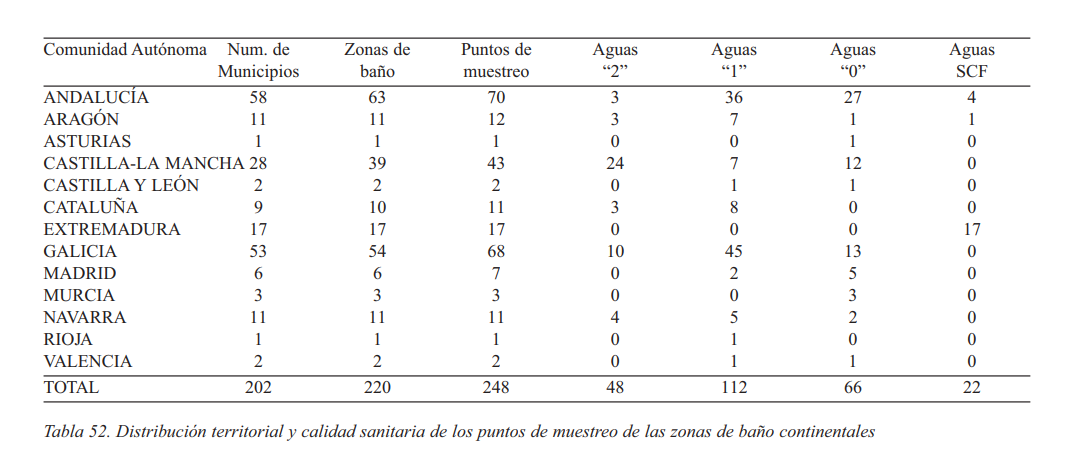
\includegraphics[width=6.25in,height=\textheight]{INPUT/images/imagenPDFTabla.png}

Para poder obtener esta tabla y poder utilizarla para el estudio,
primero se convierte el contenido del PDF a texto y luego selecciona un
rango específico de líneas en una página particular del documento
(página 17), con el objetivo de obtener datos clave relacionados con la
calidad del agua.

\begin{Shaded}
\begin{Highlighting}[]
\NormalTok{ruta\_pdf }\OtherTok{\textless{}{-}} \FunctionTok{pdf\_text}\NormalTok{(}\StringTok{"INPUT/data/report\_Cap.3\_part2.\_Libro\_blanco\_del\_agua.pdf"}\NormalTok{)}
\NormalTok{pagina }\OtherTok{\textless{}{-}}\NormalTok{ ruta\_pdf[}\DecValTok{17}\NormalTok{]}
\NormalTok{lineas }\OtherTok{\textless{}{-}} \FunctionTok{strsplit}\NormalTok{(pagina, }\StringTok{"}\SpecialCharTok{\textbackslash{}n}\StringTok{"}\NormalTok{)[[}\DecValTok{1}\NormalTok{]]}
\NormalTok{linea\_deseada }\OtherTok{\textless{}{-}}\NormalTok{ lineas[}\DecValTok{5}\SpecialCharTok{:}\DecValTok{21}\NormalTok{] }
\end{Highlighting}
\end{Shaded}

En este código se dividen las líneas deseadas usando espacios como
delimitadores. Luego, crea dos conjuntos de datos: ``datos\_obtenidos'',
excluyendo las primeras tres dimensiones no necesarias, y
``datosDeInteres'', que contiene la información esencial sobre las
comunidades autónomas y los valores de la calidad del agua.

Además, se añaden manualmente filas específicas que no se extrajeron
correctamente del informe.

\begin{Shaded}
\begin{Highlighting}[]
\NormalTok{datos\_divididos }\OtherTok{\textless{}{-}} \FunctionTok{strsplit}\NormalTok{(linea\_deseada, }\StringTok{"}\SpecialCharTok{\textbackslash{}\textbackslash{}}\StringTok{s+"}\NormalTok{)}
\NormalTok{datos\_obtenidos }\OtherTok{\textless{}{-}}\NormalTok{ datos\_divididos[}\SpecialCharTok{{-}}\FunctionTok{c}\NormalTok{(}\DecValTok{1}\SpecialCharTok{:}\DecValTok{3}\NormalTok{)]}

\NormalTok{datosDeInteres }\OtherTok{\textless{}{-}}\NormalTok{ datos\_obtenidos[}\SpecialCharTok{{-}}\FunctionTok{c}\NormalTok{(}\FunctionTok{length}\NormalTok{(datos\_obtenidos))]}
\NormalTok{datosDeInteres[[}\DecValTok{4}\NormalTok{]] }\OtherTok{\textless{}{-}} \FunctionTok{c}\NormalTok{(}\StringTok{"CASTILLA {-} LA MANCHA"}\NormalTok{,}\StringTok{"28"}\NormalTok{,}\StringTok{"39"}\NormalTok{,}\StringTok{"43"}\NormalTok{,}\StringTok{"24"}\NormalTok{,}\StringTok{"7"}\NormalTok{,}\StringTok{"12"}\NormalTok{,}\StringTok{"0"}\NormalTok{)}
\NormalTok{datosDeInteres[[}\DecValTok{5}\NormalTok{]] }\OtherTok{\textless{}{-}} \FunctionTok{c}\NormalTok{(}\StringTok{"CASTILLA Y LEÓN"}\NormalTok{,}\StringTok{"2"}\NormalTok{,}\StringTok{"2"}\NormalTok{,}\StringTok{"2"}\NormalTok{,}\StringTok{"0"}\NormalTok{,}\StringTok{"1"}\NormalTok{,}\StringTok{"1"}\NormalTok{,}\StringTok{"0"}\NormalTok{)}
\NormalTok{datosDeInteres[[}\DecValTok{9}\NormalTok{]] }\OtherTok{\textless{}{-}} \FunctionTok{c}\NormalTok{(}\StringTok{"MADRID, COMUNIDAD DE"}\NormalTok{,}\StringTok{"6"}\NormalTok{,}\StringTok{"6"}\NormalTok{,}\StringTok{"7"}\NormalTok{,}\StringTok{"0"}\NormalTok{,}\StringTok{"2"}\NormalTok{,}\StringTok{"5"}\NormalTok{,}\StringTok{"0"}\NormalTok{)}
\NormalTok{datosDeInteres[[}\DecValTok{10}\NormalTok{]] }\OtherTok{\textless{}{-}} \FunctionTok{c}\NormalTok{(}\StringTok{"MURCIA, REGIÓN DE"}\NormalTok{,}\StringTok{"3"}\NormalTok{,}\StringTok{"3"}\NormalTok{,}\StringTok{"3"}\NormalTok{,}\StringTok{"0"}\NormalTok{,}\StringTok{"0"}\NormalTok{,}\StringTok{"3"}\NormalTok{,}\StringTok{"0"}\NormalTok{)}
\NormalTok{datosDeInteres[[}\DecValTok{11}\NormalTok{]] }\OtherTok{\textless{}{-}} \FunctionTok{c}\NormalTok{(}\StringTok{"NAVARRA, COMUNIDAD FORAL DE"}\NormalTok{,}\StringTok{"11"}\NormalTok{,}\StringTok{"11"}\NormalTok{,}\StringTok{"11"}\NormalTok{,}\StringTok{"4"}\NormalTok{,}\StringTok{"5"}\NormalTok{,}\StringTok{"2"}\NormalTok{,}\StringTok{"0"}\NormalTok{)}
\NormalTok{datosDeInteres[[}\DecValTok{12}\NormalTok{]] }\OtherTok{\textless{}{-}} \FunctionTok{c}\NormalTok{(}\StringTok{"RIOJA, LA"}\NormalTok{,}\StringTok{"1"}\NormalTok{,}\StringTok{"1"}\NormalTok{,}\StringTok{"1"}\NormalTok{,}\StringTok{"0"}\NormalTok{,}\StringTok{"1"}\NormalTok{,}\StringTok{"0"}\NormalTok{,}\StringTok{"0"}\NormalTok{)}
\NormalTok{datosDeInteres[[}\DecValTok{13}\NormalTok{]] }\OtherTok{\textless{}{-}} \FunctionTok{c}\NormalTok{(}\StringTok{"COMUNITAT VALENCIANA"}\NormalTok{,}\StringTok{"2"}\NormalTok{,}\StringTok{"2"}\NormalTok{,}\StringTok{"2"}\NormalTok{,}\StringTok{"0"}\NormalTok{,}\StringTok{"1"}\NormalTok{,}\StringTok{"1"}\NormalTok{,}\StringTok{"0"}\NormalTok{)}
\end{Highlighting}
\end{Shaded}

En cada iteración del bucle, se agrega la fila representada por el
elemento i al data frame ``tablaCalidadDeAgua'' utilizando la función
\emph{rbind}( ).

Por último se renombra y se cambia a tipo numérico a aquellas columnas
que sea necesario.

\begin{Shaded}
\begin{Highlighting}[]
\NormalTok{tablaCalidadDeAgua}\OtherTok{\textless{}{-}}\FunctionTok{data.frame}\NormalTok{()}
\ControlFlowTok{for}\NormalTok{ (i }\ControlFlowTok{in}\NormalTok{ datosDeInteres)\{}
\NormalTok{  tablaCalidadDeAgua}\OtherTok{\textless{}{-}}\FunctionTok{rbind}\NormalTok{(tablaCalidadDeAgua,i)}
\NormalTok{\}}

\FunctionTok{colnames}\NormalTok{(tablaCalidadDeAgua) }\OtherTok{\textless{}{-}} \FunctionTok{c}\NormalTok{(}\StringTok{"ComunidadAutonoma"}\NormalTok{, }\StringTok{"NumdeMunicipios"}\NormalTok{, }\StringTok{"ZonasdeBaño"}\NormalTok{,}\StringTok{"PuntosdeMuestreo"}\NormalTok{,}\StringTok{"Aguas2"}\NormalTok{, }\StringTok{"Aguas1"}\NormalTok{,}\StringTok{"Aguas0"}\NormalTok{, }\StringTok{"AguasSCF"}\NormalTok{)}

\NormalTok{colNumericas }\OtherTok{\textless{}{-}} \FunctionTok{c}\NormalTok{(}\StringTok{"NumdeMunicipios"}\NormalTok{, }\StringTok{"ZonasdeBaño"}\NormalTok{,}\StringTok{"PuntosdeMuestreo"}\NormalTok{,}\StringTok{"Aguas2"}\NormalTok{, }\StringTok{"Aguas1"}\NormalTok{,}\StringTok{"Aguas0"}\NormalTok{, }\StringTok{"AguasSCF"}\NormalTok{)}
\NormalTok{tablaCalidadDeAguaFinal }\OtherTok{\textless{}{-}}\NormalTok{ tablaCalidadDeAgua }\SpecialCharTok{\%\textgreater{}\%}
  \FunctionTok{mutate\_at}\NormalTok{(}\FunctionTok{vars}\NormalTok{(colNumericas), as.integer) }\SpecialCharTok{\%\textgreater{}\%}
  \FunctionTok{select}\NormalTok{(ComunidadAutonoma, Aguas2, Aguas1, Aguas0)}
\end{Highlighting}
\end{Shaded}

\hypertarget{VariableAgua}{}

\begin{Shaded}
\begin{Highlighting}[]
\NormalTok{tablaCalidadDeAguaFinal}
\end{Highlighting}
\end{Shaded}

\begin{verbatim}
##              ComunidadAutonoma Aguas2 Aguas1 Aguas0
## 1                    ANDALUCÍA      3     36     27
## 2                       ARAGÓN      3      7      1
## 3                     ASTURIAS      0      0      1
## 4         CASTILLA - LA MANCHA     24      7     12
## 5              CASTILLA Y LEÓN      0      1      1
## 6                     CATALUÑA      3      8      0
## 7                  EXTREMADURA      0      0      0
## 8                      GALICIA     10     45     13
## 9         MADRID, COMUNIDAD DE      0      2      5
## 10           MURCIA, REGIÓN DE      0      0      3
## 11 NAVARRA, COMUNIDAD FORAL DE      4      5      2
## 12                   RIOJA, LA      0      1      0
## 13        COMUNITAT VALENCIANA      0      1      1
\end{verbatim}

En esta tabla final se pueden observar unas columnas llamadas
``Aguas1'', ``Aguas2'' y ``Aguas0'', vamos a ver a qué se refieren:

\begin{itemize}
\item
  Aguas2: Aguas aptas, de muy buena calidad.
\item
  Aguas1: Aguas aptas, de buena calidad.
\item
  Aguas0: Aguas no aptas, mala calidad.
\end{itemize}

Están evaluados diferentes puntos de muestreo en cada Comunidad
Autónoma, de los cuales se puede observar la calidad general de cada
comunidad en concreto.

\hypertarget{tabla-de-presupuesto-para-la-potabilizaciuxf3n-del-agua}{%
\subsubsection{4.4. Tabla de Presupuesto para la Potabilización del
Agua}\label{tabla-de-presupuesto-para-la-potabilizaciuxf3n-del-agua}}

Para obtener esta tabla se ha importado un archivo CSV utilizando la
función \emph{read\_csv( )} y después se renombran las columnas para
tener unificados todos los nombres de las diferentes tablas.

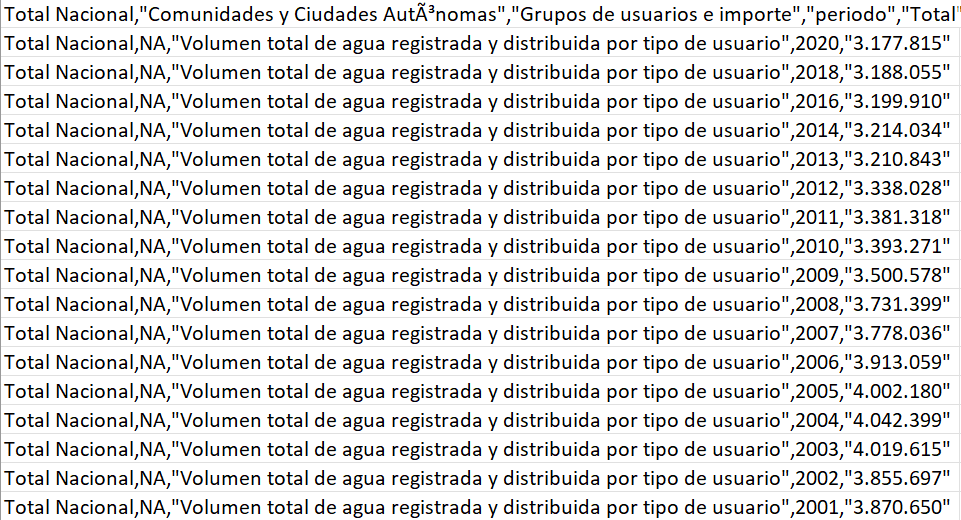
\includegraphics[width=5.20833in,height=\textheight]{INPUT/images/PresupuestoCSV.png}

Esto es una porción de todo el archivo CSV, del cual se tiene que
seleccionar los datos deseados.

Una vez cargados los datos, se renombran las columnas para poder tener
unificados todos los nombres.

\begin{Shaded}
\begin{Highlighting}[]
\NormalTok{summodificado }\OtherTok{\textless{}{-}} \FunctionTok{read\_csv}\NormalTok{(}\StringTok{"INPUT/data/summodificado.csv"}\NormalTok{)}
\FunctionTok{colnames}\NormalTok{(summodificado) }\OtherTok{\textless{}{-}} \FunctionTok{c}\NormalTok{(}\StringTok{"TotalNacional"}\NormalTok{, }\StringTok{"ComunidadAutonoma"}\NormalTok{, }\StringTok{"GruposDeUsuarioEImporte"}\NormalTok{,}\StringTok{"Anio"}\NormalTok{, }\StringTok{"Presupuesto"}\NormalTok{)}
\end{Highlighting}
\end{Shaded}

Se seleccionan las filas donde la columna ``GruposDeUsuarioEImporte'' es
igual a ``Importe total de la inversión en los servicios de suministro''
y la columna ``Anio'' es igual a ``2020''.

Delante de cada nombre de la Comunidad Autónoma existe un número por lo
que se elimina y se convierten los nombres de las comunidades a
mayúsculas.

Se eliminan los puntos de la columna presupuesto y se pasa a tipo
entero. Y por último se descarta lo que no es necesario.

\begin{Shaded}
\begin{Highlighting}[]
\NormalTok{tablaPresupuestos }\OtherTok{\textless{}{-}}\NormalTok{ summodificado}\SpecialCharTok{\%\textgreater{}\%}
  \FunctionTok{filter}\NormalTok{(GruposDeUsuarioEImporte}\SpecialCharTok{==}\StringTok{"Importe total de la inversión en los servicios de suministro"} \SpecialCharTok{\&}\NormalTok{ Anio}\SpecialCharTok{==} \StringTok{"2020"}\NormalTok{) }\SpecialCharTok{\%\textgreater{}\%}
  \FunctionTok{mutate}\NormalTok{(}\AttributeTok{ComunidadAutonoma =} \FunctionTok{gsub}\NormalTok{(}\StringTok{"\^{}}\SpecialCharTok{\textbackslash{}\textbackslash{}}\StringTok{d+}\SpecialCharTok{\textbackslash{}\textbackslash{}}\StringTok{s*"}\NormalTok{, }\StringTok{""}\NormalTok{, ComunidadAutonoma)) }\SpecialCharTok{\%\textgreater{}\%}
  \FunctionTok{mutate}\NormalTok{(}\AttributeTok{ComunidadAutonoma =} \FunctionTok{toupper}\NormalTok{(ComunidadAutonoma)) }\SpecialCharTok{\%\textgreater{}\%}
  \FunctionTok{select}\NormalTok{ (}\AttributeTok{.data =}\NormalTok{ ., Anio, ComunidadAutonoma}\SpecialCharTok{:}\NormalTok{Presupuesto) }\SpecialCharTok{\%\textgreater{}\%}
  \FunctionTok{drop\_na}\NormalTok{()}

\NormalTok{tablaPresupuestos}\SpecialCharTok{$}\NormalTok{Presupuesto }\OtherTok{\textless{}{-}} \FunctionTok{gsub}\NormalTok{(}\StringTok{"}\SpecialCharTok{\textbackslash{}\textbackslash{}}\StringTok{."}\NormalTok{, }\StringTok{""}\NormalTok{, tablaPresupuestos}\SpecialCharTok{$}\NormalTok{Presupuesto)}
\NormalTok{tablaPresupuestos}\SpecialCharTok{$}\NormalTok{Presupuesto }\OtherTok{\textless{}{-}} \FunctionTok{as.integer}\NormalTok{(tablaPresupuestos}\SpecialCharTok{$}\NormalTok{Presupuesto)}
\NormalTok{tablaPresupuestosFinal }\OtherTok{\textless{}{-}}\NormalTok{ tablaPresupuestos[,}\SpecialCharTok{{-}}\DecValTok{3}\NormalTok{]}
\end{Highlighting}
\end{Shaded}

Asi obtenemos los datos de los presupuesto para la potabilización del
agua en el año 2020 en las diferentes Comunidades Autónomas de España

\begin{Shaded}
\begin{Highlighting}[]
\NormalTok{tablaPresupuestosFinal}
\end{Highlighting}
\end{Shaded}

\begin{verbatim}
## # A tibble: 17 x 3
##     Anio ComunidadAutonoma           Presupuesto
##    <dbl> <chr>                             <int>
##  1  2020 ANDALUCÍA                         43361
##  2  2020 ARAGÓN                              691
##  3  2020 ASTURIAS, PRINCIPADO DE             757
##  4  2020 BALEARS, ILLES                    14514
##  5  2020 CANARIAS                           4015
##  6  2020 CANTABRIA                           223
##  7  2020 CASTILLA Y LEÓN                    8083
##  8  2020 CASTILLA - LA MANCHA               2397
##  9  2020 CATALUÑA                          30222
## 10  2020 COMUNITAT VALENCIANA              39274
## 11  2020 EXTREMADURA                        2263
## 12  2020 GALICIA                            2594
## 13  2020 MADRID, COMUNIDAD DE              80532
## 14  2020 MURCIA, REGIÓN DE                  3170
## 15  2020 NAVARRA, COMUNIDAD FORAL DE        5704
## 16  2020 PAÍS VASCO                         3001
## 17  2020 RIOJA, LA                           304
\end{verbatim}

\hypertarget{joins-y-gruxe1ficas}{%
\section{5. Joins y Gráficas}\label{joins-y-gruxe1ficas}}

En este aparatado realizamos una cantidad de cuatro joins, los cuales
explicaremos a continuación.

\hypertarget{relaciuxf3n-entre-esperanza-de-vida-y-cantidad}{%
\subsubsection{5.1. Relación entre Esperanza de Vida y
Cantidad}\label{relaciuxf3n-entre-esperanza-de-vida-y-cantidad}}

\begin{Shaded}
\begin{Highlighting}[]
\NormalTok{EsperanzayCantidad}\OtherTok{\textless{}{-}}\NormalTok{ tablaEsperanzaDeVidaFinal}\SpecialCharTok{\%\textgreater{}\%}
  \FunctionTok{left\_join}\NormalTok{(}\AttributeTok{x=}\NormalTok{., }\AttributeTok{y=}\NormalTok{tablaCantidadDeAguaFinal, }\AttributeTok{by=}\FunctionTok{c}\NormalTok{(}\StringTok{"Anio"}\NormalTok{,}\StringTok{"ComunidadAutonoma"}\NormalTok{))}\SpecialCharTok{\%\textgreater{}\%}
  \FunctionTok{group\_by}\NormalTok{(ComunidadAutonoma) }\SpecialCharTok{\%\textgreater{}\%}
  \FunctionTok{drop\_na}\NormalTok{()}
\NormalTok{EsperanzayCantidad}
\end{Highlighting}
\end{Shaded}

\begin{verbatim}
## # A tibble: 16 x 4
## # Groups:   ComunidadAutonoma [16]
##     Anio ComunidadAutonoma           EsperanzaDeVida Cantidad
##    <dbl> <chr>                                 <dbl>    <dbl>
##  1  2020 ANDALUCÍA                              28.0  262867 
##  2  2020 ARAGÓN                                 28.4   38689.
##  3  2020 BALEARS, ILLES                         29.3   42033.
##  4  2020 CANARIAS                               29.1   79923.
##  5  2020 CANTABRIA                              28.9   20367.
##  6  2020 CASTILLA - LA MANCHA                   27.5   60920.
##  7  2020 CASTILLA Y LEÓN                        28.5   73272.
##  8  2020 CATALUÑA                               28.3  239767.
##  9  2020 COMUNITAT VALENCIANA                   28.5  188854.
## 10  2020 EXTREMADURA                            27.9   28064.
## 11  2020 GALICIA                                29.3   71149 
## 12  2020 MADRID, COMUNIDAD DE                   28.0  216232.
## 13  2020 MURCIA, REGIÓN DE                      28.4   57000.
## 14  2020 NAVARRA, COMUNIDAD FORAL DE            29.0   22551.
## 15  2020 PAÍS VASCO                             28.8   52635.
## 16  2020 RIOJA, LA                              28.6    9448.
\end{verbatim}

En el fragmento de código anterior, combinamos mediante un
\emph{left\_join( )} las tablas de ``tablaEsperanzaDeVidaFinal'' y
``tablaCantidadDeAguaFinal'' usando sus claves comunes, las columnas
``Anio'' y ``ComunidadAutonoma'' ordenado en función de las Comunidades
Autónomas.

\begin{Shaded}
\begin{Highlighting}[]
\NormalTok{grafEsperanzaCantidad }\OtherTok{\textless{}{-}} \FunctionTok{ggplot}\NormalTok{(}\AttributeTok{data=}\NormalTok{EsperanzayCantidad, }\FunctionTok{aes}\NormalTok{(}\AttributeTok{x=}\NormalTok{Cantidad, }\AttributeTok{y=}\NormalTok{EsperanzaDeVida))}\SpecialCharTok{+}
  \FunctionTok{geom\_point}\NormalTok{(}\FunctionTok{aes}\NormalTok{(}\AttributeTok{color=}\NormalTok{ComunidadAutonoma))}\SpecialCharTok{+}
  \FunctionTok{geom\_smooth}\NormalTok{()}\SpecialCharTok{+}
  \FunctionTok{labs}\NormalTok{(}\AttributeTok{title=}\StringTok{"Relación entre Esperanza de Vida y Cantidad"}\NormalTok{,}
       \AttributeTok{x=}\StringTok{"Cantidad de agua "}\NormalTok{,}
       \AttributeTok{y=}\StringTok{"Esperanza de vida"}\NormalTok{)}\SpecialCharTok{+}
  \FunctionTok{theme\_minimal}\NormalTok{()}
\NormalTok{grafEsperanzaCantidad}
\end{Highlighting}
\end{Shaded}

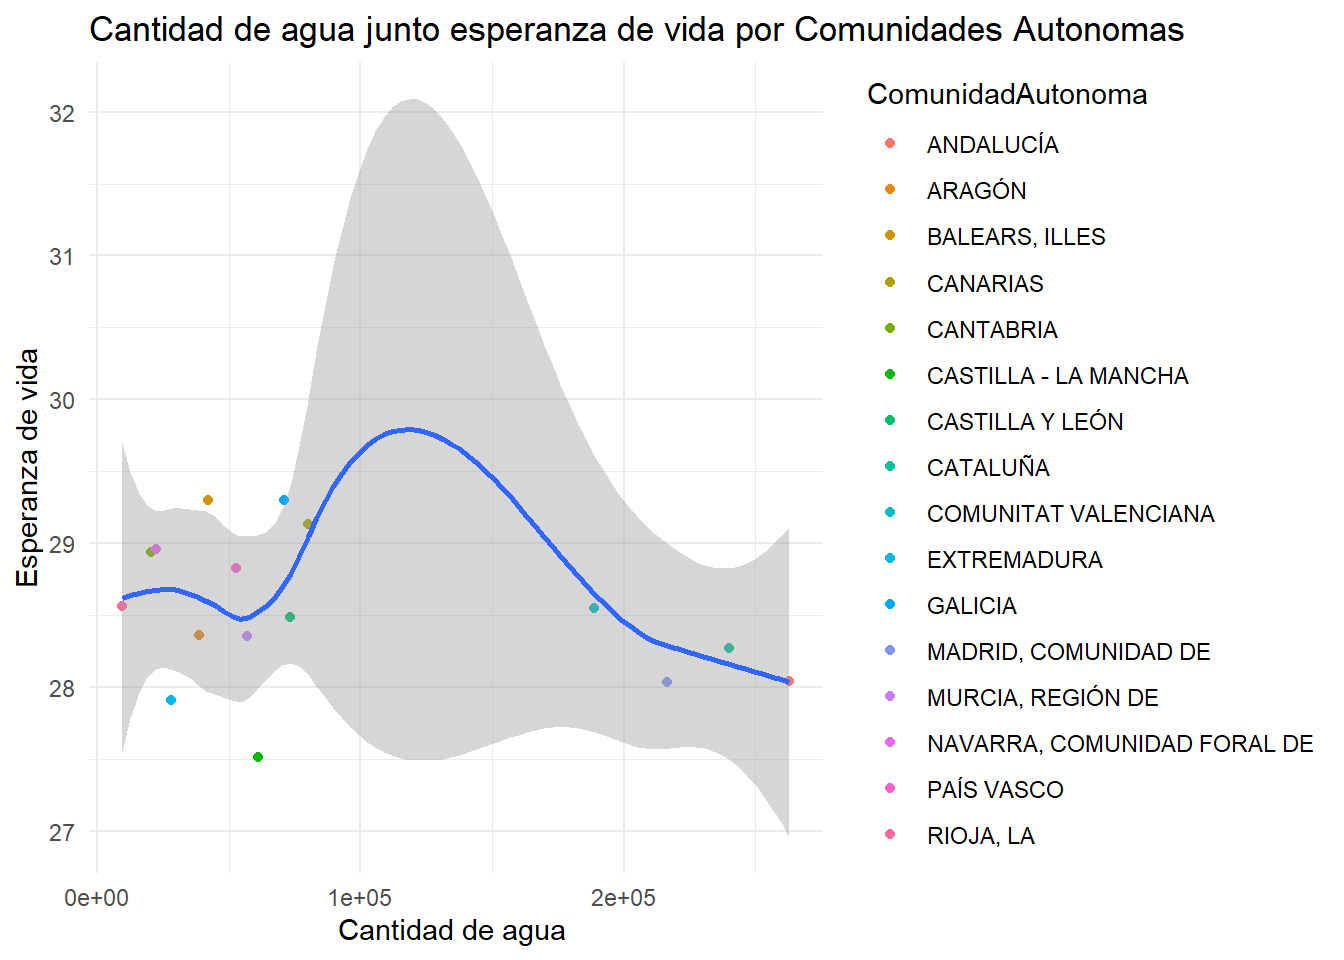
\includegraphics{Seminario_UrkoPaulaVictoria_files/figure-latex/grafEsperanzaCantidad-1.pdf}

Como podemos observar en esta caja de código, creamos la gráfica de la
nueva tabla ``EsperanzayCantidad'', creada a partir del
\emph{left\_join( )} anterior. En el eje de las abscisas se representa
la cantidad de agua consumida, mientras que en el eje de las ordenadas
encontramos la esperanza de vida. La leyenda muestra que cada comunidad
es representada en la gráfica mediante un color del gradiente y en forma
circular gracias a la función
``\emph{geom\_point(aes(color=ComunidadAutonoma))``}. Con la funcion
\emph{geom\_smooth()} creamos la línea de tendencia, ya que tenemos un
gráfico de dispersión y así podemos entender el patrón que estamos
estudiando con esta gráfica.

Nuestro principal objetivo es determinar la esperanza de vida. En esta
tabla relacionamos la esperanza de vida con la cantidad de agua que se
consume en cada Comunidad Autónoma. Podemos observar que no hay una
relación directamente proporcional entre la cantidad de agua consumida y
la esperanza de vida de cada Comunidad Autónoma. Comprobamos en el
\protect\hyperlink{anexo}{Anexo I} que las Islas Baleares se encuentra
en la undécima posición en cuanto al consumo de agua (42033.429) y en
primer lugar en cuanto a la esperanza de vida (29,29776). Por otro lado,
Andalucía está situada en el primer puesto en cuanto a la cantidad de
agua que consumen (262867.000) y en el decimotercero en lo que respecta
a la esperanza de vida (28.03881). Sin embargo, al observar la línea de
tendencia de nuestro gráfico, notamos que los extremos no son lo ideal.
Por lo tanto, la tendencia nos sugiere que aquellos ciudadanos con una
esperanza de vida potencialmente alta son aquellos que consumen una
cantidad intermedia de agua.

\hypertarget{relaciuxf3n-entre-cantidad-y-presupuesto}{%
\subsubsection{5.2. Relación entre Cantidad y
Presupuesto}\label{relaciuxf3n-entre-cantidad-y-presupuesto}}

\begin{Shaded}
\begin{Highlighting}[]
\NormalTok{CantidadyPresupuesto}\OtherTok{\textless{}{-}}\NormalTok{ tablaCantidadDeAguaFinal}\SpecialCharTok{\%\textgreater{}\%} 
  \FunctionTok{left\_join}\NormalTok{(}\AttributeTok{x=}\NormalTok{., }\AttributeTok{y=}\NormalTok{tablaPresupuestosFinal, }\AttributeTok{by=}\FunctionTok{c}\NormalTok{(}\StringTok{"Anio"}\NormalTok{,}\StringTok{"ComunidadAutonoma"}\NormalTok{)) }\SpecialCharTok{\%\textgreater{}\%} 
  \FunctionTok{arrange}\NormalTok{(}\FunctionTok{desc}\NormalTok{(Presupuesto)) }\SpecialCharTok{\%\textgreater{}\%}
  \FunctionTok{drop\_na}\NormalTok{()}
\NormalTok{CantidadyPresupuesto}
\end{Highlighting}
\end{Shaded}

\begin{verbatim}
## # A tibble: 16 x 4
## # Groups:   Anio [1]
##     Anio ComunidadAutonoma           Cantidad Presupuesto
##    <dbl> <chr>                          <dbl>       <int>
##  1  2020 MADRID, COMUNIDAD DE         216232.       80532
##  2  2020 ANDALUCÍA                    262867        43361
##  3  2020 COMUNITAT VALENCIANA         188854.       39274
##  4  2020 CATALUÑA                     239767.       30222
##  5  2020 BALEARS, ILLES                42033.       14514
##  6  2020 CASTILLA Y LEÓN               73272.        8083
##  7  2020 NAVARRA, COMUNIDAD FORAL DE   22551.        5704
##  8  2020 CANARIAS                      79923.        4015
##  9  2020 MURCIA, REGIÓN DE             57000.        3170
## 10  2020 PAÍS VASCO                    52635.        3001
## 11  2020 GALICIA                       71149         2594
## 12  2020 CASTILLA - LA MANCHA          60920.        2397
## 13  2020 EXTREMADURA                   28064.        2263
## 14  2020 ARAGÓN                        38689.         691
## 15  2020 RIOJA, LA                      9448.         304
## 16  2020 CANTABRIA                     20367.         223
\end{verbatim}

En el fragmento de código anterior, combinamos a través de un
\emph{left\_join( )} las tablas de ``tablaCantidadDeAguaFinal'' y
``tablaPresupuestosFinal'' gracias a sus claves comunes ``Anio'' y
``ComunidadAutonoma'', ordenadas en función de las del presupuesto de
manera descendente.

\begin{Shaded}
\begin{Highlighting}[]
\NormalTok{grafCantidadPresupuesto }\OtherTok{\textless{}{-}} \FunctionTok{ggplot}\NormalTok{(}\AttributeTok{data=}\NormalTok{CantidadyPresupuesto, }\FunctionTok{aes}\NormalTok{(}\AttributeTok{x=}\NormalTok{ Presupuesto, }\AttributeTok{y=}\NormalTok{ Cantidad, }\AttributeTok{fill=}\NormalTok{ComunidadAutonoma))}\SpecialCharTok{+}
  \FunctionTok{geom\_bar}\NormalTok{(}\AttributeTok{stat=} \StringTok{"identity"}\NormalTok{)}\SpecialCharTok{+}
  \FunctionTok{labs}\NormalTok{(}\AttributeTok{title=}\StringTok{"Relación entre Cantidad y Presupuesto"}\NormalTok{,}
       \AttributeTok{x=}\StringTok{"Presupuestos"}\NormalTok{,}
       \AttributeTok{y=}\StringTok{"Cantidad de agua"}\NormalTok{)}\SpecialCharTok{+}
  \FunctionTok{geom\_bar}\NormalTok{(}\AttributeTok{stat=} \StringTok{"identity"}\NormalTok{, }\AttributeTok{width =} \DecValTok{5000}\NormalTok{)}\SpecialCharTok{+}
  \FunctionTok{theme\_minimal}\NormalTok{()}
\NormalTok{grafCantidadPresupuesto}
\end{Highlighting}
\end{Shaded}

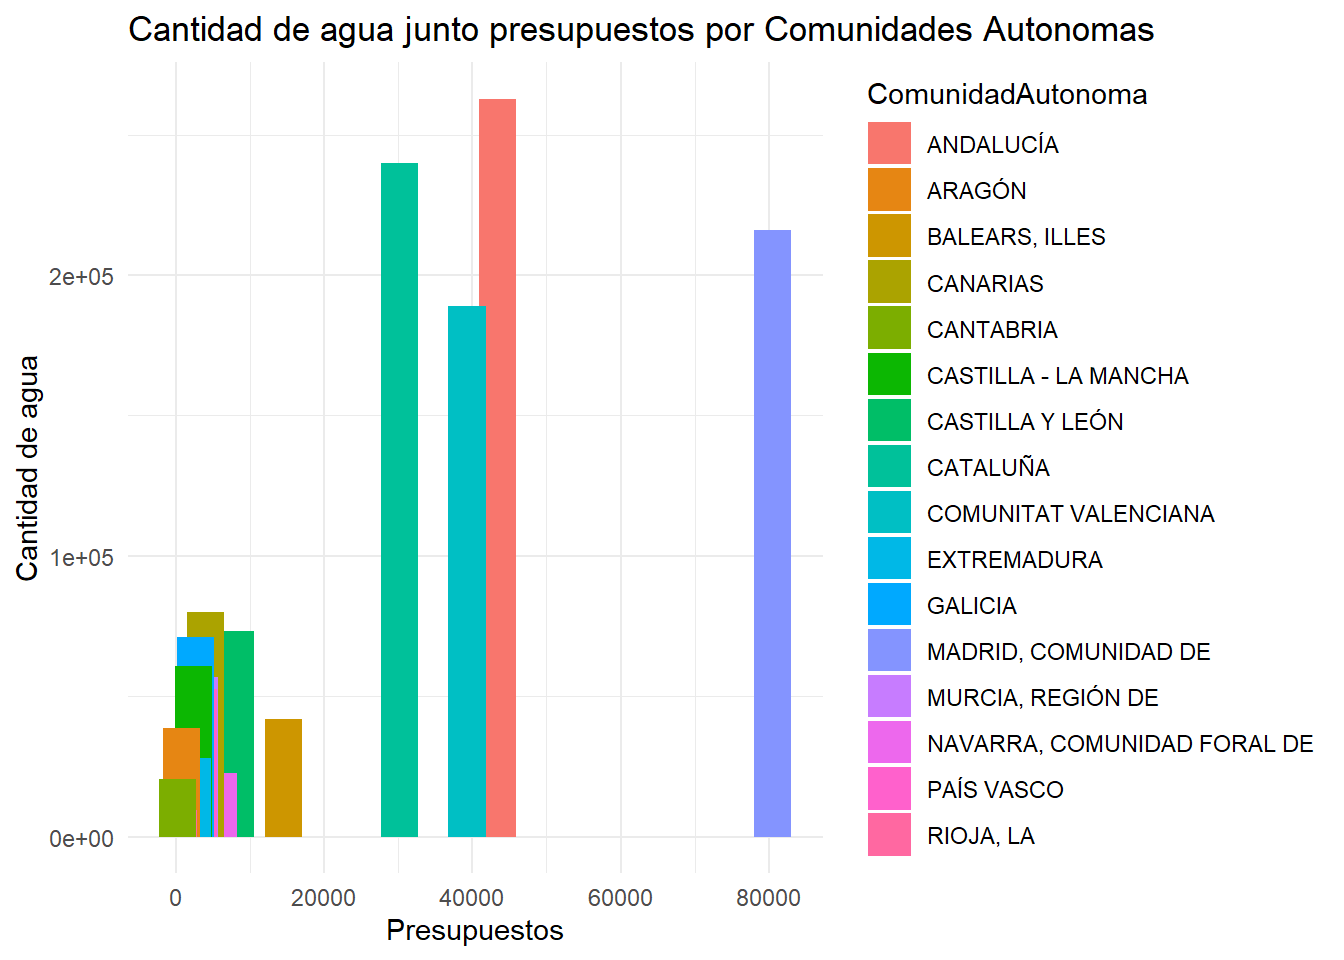
\includegraphics{Seminario_UrkoPaulaVictoria_files/figure-latex/grafCantidadPresupuesto-1.pdf}

Aquí creamos la gráfica de la nueva tabla ``grafCantidadPresupuesto'',
creada a partir del \emph{left\_join( )} anterior. En el eje de las
ordenadas encontramos la cantidad de agua consumida, y en el eje de las
abscisas encontramos los presupuestos. Como podemos comprobar en la
leyenda, gracias a la función \emph{(\ldots)fill=ComunidadAutonoma))+
geom\_bar(stat= ``identity'')}, cada comunidad será representada en la
gráfica por un color perteneciente al gradiente y en forma de barra.

Al observar la tabla y el gráfico, es evidente que en este caso sí
podemos apreciar una correlación significativa entre el prespuesto
invertido en agua y su consumo. Lugares como la Comunidad de Madrid,
Andalucía o la Comunidad Valenciana encabezan los presupuestos más altos
y el consumo de agua mayor (puede comprobarese en el
\protect\hyperlink{CantidadPresupuesto}{Anexo I} ). Por otro lado, La
Rioja , Cantabria, Extremadura y Aragón, rondan los últimos puestos
tanto en presupuesto como en cantidad. Podemos destacar Castilla-La
Mancha, que con un gasto relativamente bajo en agua, tienen un consumo
considerable, justo lo contrario de la Comunidad Foral de Navarra. Aun
teniendo en cuenta las pocas comunidades que no se rigen por la
normalidad de este gráfico, podemos afirmar que una mayor inversión por
parte de las Comunidades Autónomas fomentan un mayor consumo de agua en
sus habitantes.

\hypertarget{relaciuxf3n-entre-esperanza-de-vida-y-calidad}{%
\subsubsection{5.3. Relación entre Esperanza de Vida y
Calidad}\label{relaciuxf3n-entre-esperanza-de-vida-y-calidad}}

\begin{Shaded}
\begin{Highlighting}[]
\NormalTok{EsperanzayCalidad}\OtherTok{\textless{}{-}}\NormalTok{ tablaEsperanzaDeVidaFinal}\SpecialCharTok{\%\textgreater{}\%}
  \FunctionTok{left\_join}\NormalTok{(}\AttributeTok{x=}\NormalTok{., }\AttributeTok{y=}\NormalTok{tablaCalidadDeAguaFinal, }\AttributeTok{by=}\FunctionTok{c}\NormalTok{(}\StringTok{"ComunidadAutonoma"}\NormalTok{))}\SpecialCharTok{\%\textgreater{}\%}
  \FunctionTok{group\_by}\NormalTok{(ComunidadAutonoma) }\SpecialCharTok{\%\textgreater{}\%}
  \FunctionTok{drop\_na}\NormalTok{()}
\NormalTok{EsperanzayCalidadFinal }\OtherTok{\textless{}{-}} \FunctionTok{pivot\_longer}\NormalTok{(}\AttributeTok{data =}\NormalTok{ EsperanzayCalidad, }\AttributeTok{names\_to =} \StringTok{"CalidadAgua"}\NormalTok{, }\AttributeTok{values\_to =} \StringTok{"ValoresCalidadAgua"}\NormalTok{, }\AttributeTok{cols =} \FunctionTok{c}\NormalTok{(Aguas2,Aguas1,Aguas0))}

\NormalTok{EsperanzayCalidadFinal}
\end{Highlighting}
\end{Shaded}

\begin{verbatim}
## # A tibble: 36 x 5
## # Groups:   ComunidadAutonoma [12]
##     Anio ComunidadAutonoma    EsperanzaDeVida CalidadAgua ValoresCalidadAgua
##    <dbl> <chr>                          <dbl> <chr>                    <int>
##  1  2020 ANDALUCÍA                       28.0 Aguas2                       3
##  2  2020 ANDALUCÍA                       28.0 Aguas1                      36
##  3  2020 ANDALUCÍA                       28.0 Aguas0                      27
##  4  2020 ARAGÓN                          28.4 Aguas2                       3
##  5  2020 ARAGÓN                          28.4 Aguas1                       7
##  6  2020 ARAGÓN                          28.4 Aguas0                       1
##  7  2020 CASTILLA - LA MANCHA            27.5 Aguas2                      24
##  8  2020 CASTILLA - LA MANCHA            27.5 Aguas1                       7
##  9  2020 CASTILLA - LA MANCHA            27.5 Aguas0                      12
## 10  2020 CASTILLA Y LEÓN                 28.5 Aguas2                       0
## # i 26 more rows
\end{verbatim}

En este código, combinamos con un \emph{left\_join( )} las tablas de
``tablaEsperanzaDeVidaFinal'' y ``tablaCalidadDeAguaFinal'' mediante su
clave común, la columna ``ComunidadAutonoma'', ordenado en función de la
Comunidad Autónoma . De esta tabla, consideraremos las columnas
``Aguas2'', ``Aguas1'', ``Aguas 0'', las cuales son relevantes en
nuestro estudio.

Gracias a un \emph{pivot\_longer( ),} podemos crear una nueva columna
``CalidadAgua'', agrupando las tres últimas columnas en distintas filas,
y otra columna ``ValoresCalidadAgua'' con los valores correspondientes a
esas variables, haciendo más fácil su posterior estudio en la gráfica.

\begin{Shaded}
\begin{Highlighting}[]
\NormalTok{grafEsperanzaCalidad }\OtherTok{\textless{}{-}} \FunctionTok{ggplot}\NormalTok{(}\AttributeTok{data =}\NormalTok{ EsperanzayCalidadFinal, }\FunctionTok{aes}\NormalTok{(}\AttributeTok{x =}\NormalTok{ ValoresCalidadAgua, }\AttributeTok{y =}\NormalTok{ EsperanzaDeVida)) }\SpecialCharTok{+}
  \FunctionTok{geom\_point}\NormalTok{(}\FunctionTok{aes}\NormalTok{(}\AttributeTok{colour =}\NormalTok{ ComunidadAutonoma)) }\SpecialCharTok{+}
  \FunctionTok{facet\_wrap}\NormalTok{(}\AttributeTok{facets =} \FunctionTok{vars}\NormalTok{(CalidadAgua), }\AttributeTok{nrow =} \DecValTok{1}\NormalTok{)}\SpecialCharTok{+}
  \FunctionTok{labs}\NormalTok{(}\AttributeTok{title=}\StringTok{"Relación entre Esperanza de Vida y Calidad"}\NormalTok{,}
       \AttributeTok{x=}\StringTok{"Calidad"}\NormalTok{,}
       \AttributeTok{y=}\StringTok{"Esperanza de vida"}\NormalTok{)}\SpecialCharTok{+}
  \FunctionTok{theme\_minimal}\NormalTok{()}
\NormalTok{grafEsperanzaCalidad}
\end{Highlighting}
\end{Shaded}

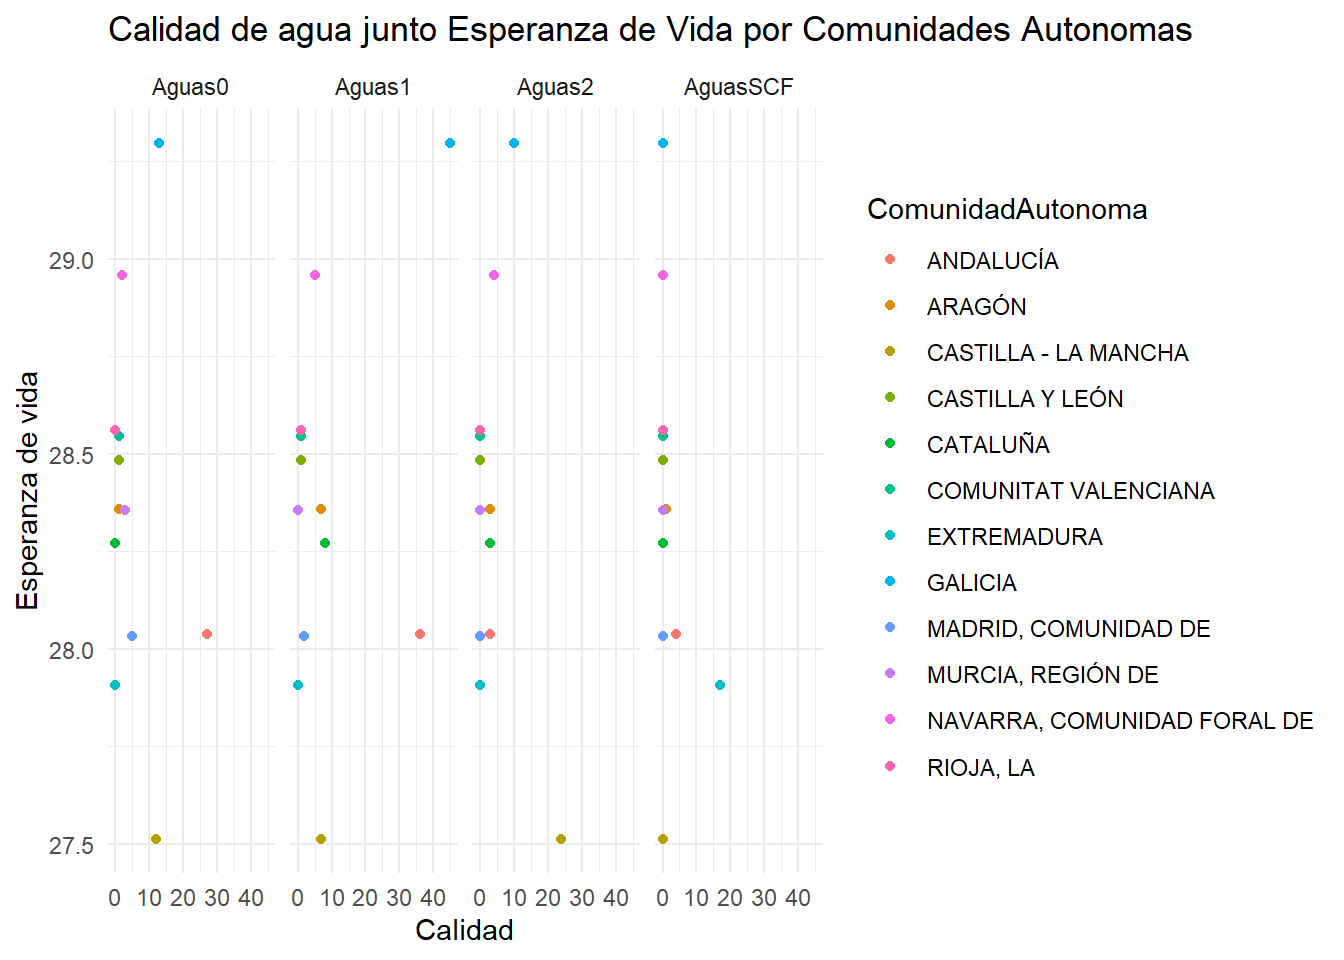
\includegraphics{Seminario_UrkoPaulaVictoria_files/figure-latex/grafEsperanzaCalidad-1.pdf}

Para crear este gráfico a partir de la nueva tabla
``CalidadyEsperanza'', utilizamos como eje de abscisas la variable
``ValoresCalidadAgua'', mientras que de eje de ordenadas se encuetra la
variable ``EsperanzaDeVida''. Por medio de la funcion \emph{geom\_point(
),} agregamos puntos al gráfico asignando colores en función de la
Comunidad Autónoma que represente. Al tener varios datos de la calidad
del agua, dividimos las facetas con la ayuda de la función
\emph{facet\_wrap( )} organizándolas en una sola fila.

Como se explica en el \protect\hyperlink{VariableAgua}{Apartado 3 de la
obtención de tablas}, los tres tipos de agua nos indicarán el grado de
calidad de estas. Según los porcentajes obtenidos en el
\protect\hyperlink{tablaPorcentaje}{Anexo}\protect\hyperlink{anexo}{I},
la Comunidad Autónoma que utiliza como fuente principial las aguas de
tipo ``Aguas 2'' es Castilla La Mancha, pero su esperaza de vida es
baja. Luego, Comunidades Autónomas como Murcia y Asturias utilizan el
100\% de ``Aguas 0'' y aun así tienen una esperanza de vida en la media
de lo normal. Por último, Galicia, líder en esperanza de vida, usa en su
mayoría aguas de tipo ``Aguas 1''. Concluyendo así que no hay ninguna
relación a primera vista sobre la calidad de agua utilizada y la
esperanza de vida.

\hypertarget{relaciuxf3n-entre-esperanza-de-vida-calidad-presupuesto-y-cantidad.}{%
\subsubsection{5.4. Relación entre Esperanza de Vida, Calidad,
Presupuesto y
Cantidad.}\label{relaciuxf3n-entre-esperanza-de-vida-calidad-presupuesto-y-cantidad.}}

\begin{Shaded}
\begin{Highlighting}[]
\NormalTok{tablaend}\OtherTok{\textless{}{-}}\NormalTok{ EsperanzayCantidad }\SpecialCharTok{\%\textgreater{}\%} 
  \FunctionTok{left\_join}\NormalTok{(}\AttributeTok{x=}\NormalTok{., }\AttributeTok{y=}\NormalTok{CantidadyPresupuesto, }\AttributeTok{by=}\FunctionTok{c}\NormalTok{(}\StringTok{"Cantidad"}\NormalTok{,}\StringTok{"ComunidadAutonoma"}\NormalTok{,}\StringTok{"Anio"}\NormalTok{)) }\SpecialCharTok{\%\textgreater{}\%}
  \FunctionTok{left\_join}\NormalTok{(}\AttributeTok{x=}\NormalTok{., }\AttributeTok{y=}\NormalTok{EsperanzayCalidadFinal, }\AttributeTok{by=}\FunctionTok{c}\NormalTok{(}\StringTok{"ComunidadAutonoma"}\NormalTok{)) }\SpecialCharTok{\%\textgreater{}\%} 
  \FunctionTok{mutate}\NormalTok{(}\AttributeTok{EsperanzaDeVida =} \FunctionTok{coalesce}\NormalTok{(EsperanzaDeVida.x, EsperanzaDeVida.y)) }\SpecialCharTok{\%\textgreater{}\%}
  \FunctionTok{select}\NormalTok{(}\SpecialCharTok{{-}}\NormalTok{EsperanzaDeVida.x, }\SpecialCharTok{{-}}\NormalTok{EsperanzaDeVida.y)}\SpecialCharTok{\%\textgreater{}\%}
  \FunctionTok{mutate}\NormalTok{(}\AttributeTok{Anio =} \FunctionTok{coalesce}\NormalTok{(Anio.x, Anio.y))}\SpecialCharTok{\%\textgreater{}\%}
  \FunctionTok{select}\NormalTok{(}\SpecialCharTok{{-}}\NormalTok{Anio.x, }\SpecialCharTok{{-}}\NormalTok{Anio.y)}\SpecialCharTok{\%\textgreater{}\%}
  \FunctionTok{select}\NormalTok{(Anio, ComunidadAutonoma, }\FunctionTok{everything}\NormalTok{())}\SpecialCharTok{\%\textgreater{}\%}
  \FunctionTok{drop\_na}\NormalTok{()}
\NormalTok{tablaend}
\end{Highlighting}
\end{Shaded}

\begin{verbatim}
## # A tibble: 36 x 7
## # Groups:   ComunidadAutonoma [12]
##     Anio ComunidadAutonoma   Cantidad Presupuesto CalidadAgua ValoresCalidadAgua
##    <dbl> <chr>                  <dbl>       <int> <chr>                    <int>
##  1  2020 ANDALUCÍA            262867        43361 Aguas2                       3
##  2  2020 ANDALUCÍA            262867        43361 Aguas1                      36
##  3  2020 ANDALUCÍA            262867        43361 Aguas0                      27
##  4  2020 ARAGÓN                38689.         691 Aguas2                       3
##  5  2020 ARAGÓN                38689.         691 Aguas1                       7
##  6  2020 ARAGÓN                38689.         691 Aguas0                       1
##  7  2020 CASTILLA - LA MANC~   60920.        2397 Aguas2                      24
##  8  2020 CASTILLA - LA MANC~   60920.        2397 Aguas1                       7
##  9  2020 CASTILLA - LA MANC~   60920.        2397 Aguas0                      12
## 10  2020 CASTILLA Y LEÓN       73272.        8083 Aguas2                       0
## # i 26 more rows
## # i 1 more variable: EsperanzaDeVida <dbl>
\end{verbatim}

En este código, unimos mediante un \emph{left\_join( )} las tablas de
``EsperanzayCantidad'' y ``CantidadyPresupuesto'' teniendo como clave
común las columnas ``ComunidadAutonoma'', ``Cantidad'' y ``Anio''.
Posteriormente, realizamos otro \emph{letf\_join( )} combinando las
tablas ``EsperanzayCantidad'' junto con ``EsperanzayCalidadFinal'', las
cuales se unen gracias a la columna ``ComunidadAutonoma'' . A partir del
resultado anterior, eliminaremos las columnas no deseadas
(``NumdeMunicipios'',``ZonasdeBaño'',``PuntosdeMuestreo'') con la
función \emph{select( ).} Por otro lado, modificaremos las columnas que
aparecen con ``.x'', recuperando su nombre original seleccionando el
primer valor no nulo.

\begin{Shaded}
\begin{Highlighting}[]
\NormalTok{grafTablaFinal }\OtherTok{\textless{}{-}} \FunctionTok{ggplot}\NormalTok{(tablaend, }\FunctionTok{aes}\NormalTok{(}\AttributeTok{x =}\NormalTok{ Cantidad, }\AttributeTok{y =}\NormalTok{ EsperanzaDeVida, }\AttributeTok{size =}\NormalTok{ Presupuesto, }\AttributeTok{color =}\NormalTok{ CalidadAgua)) }\SpecialCharTok{+}
  \FunctionTok{geom\_point}\NormalTok{() }\SpecialCharTok{+}
  \FunctionTok{labs}\NormalTok{(}\AttributeTok{title =} \StringTok{"Relación entre Cantidad, Esperanza de Vida, Presupuesto y Calidad"}\NormalTok{,      }\AttributeTok{x =} \StringTok{"Cantidad"}\NormalTok{,}
       \AttributeTok{y =} \StringTok{"Esperanza de Vida"}\NormalTok{,}
       \AttributeTok{size =} \StringTok{"Presupuesto"}\NormalTok{,}
       \AttributeTok{color =} \StringTok{"CalidadAgua"}\NormalTok{)}\SpecialCharTok{+}
      \FunctionTok{theme\_minimal}\NormalTok{()}
\NormalTok{grafTablaFinal}
\end{Highlighting}
\end{Shaded}

\includegraphics{Seminario_UrkoPaulaVictoria_files/figure-latex/grafTablaFinal-1.pdf}

En relación con el último gráfico, se puede observar la combinación de
las cuatro variables tratadas a lo largo de este seminario. Para poder
relacionarlas entre ellas, creamos un gráfico de dispersión mediante la
función \emph{geom\_point( )} . El eje de las abscisas representa la
Cantidad de agua consumida, el eje de las ordenadas representa la
Esperanza de vida, y la Calidad del Agua se encarga de proporcionar el
color a los círculos mientras que su tamaño esta determinado por el
Presupuesto. Cabe destacar que el único color visible es el morado; esto
no quiere decir que el resto de valores no esten representados, sino que
se encuentran superpuestos.

Como conclusión final, podemos ver que la relación entre presupuesto y
la cantidad de agua consumida si que es notoria. No obstante, se observa
que la esperanza de vida no se ve afectada por el presupuesto. Podemos
comprobar que los extremos en la variable de la cantidad de agua si que
perjudican a la esperanza de vida; aquellos que consumen mucha agua o
muy poca tienen una esperanza de vida relativamente inferior a los que
consumen una cantidad intermedia. Por otro lado, al superponerse los
puntos de calidad de agua, se evidencia que realmente no es una variable
que afecte directamente a nuestro estudio. Como conclusión, la esperanza
de vida tiende a ser mayor si nuestro consumo de agua no excede ningun
límite, permitiendo asi que aquellas Comunidades Autónomas que invierten
una gran cantidad en el consumo de agua puedan reducir dicha inversión.

\hypertarget{conclusiuxf3n}{%
\section{6. Conclusión}\label{conclusiuxf3n}}

A lo largo de este seminario, hemos relacionado las distintas variables
con el fin de comprobar si realmente afectan o no a la esperanza de
vida. Como conclusión, la esperanza de vida tiende a ser mayor si
nuestro consumo de agua no excede ningun límite, permitiendo asi que
aquellas Comunidades Autónomas que invierten una gran cantidad en el
consumo de agua puedan reducir dicha inversión.

\hypertarget{anexo}{%
\section{Anexo I}\label{anexo}}

\begin{itemize}
\tightlist
\item
  Orden de la tabla EsperanzayCantidad de mayor a menor en función de:
\end{itemize}

La esperanza de vida

\begin{Shaded}
\begin{Highlighting}[]
\NormalTok{EsparanzaVidaMayorMenor }\OtherTok{\textless{}{-}}\NormalTok{ EsperanzayCantidad[}\FunctionTok{order}\NormalTok{(}\SpecialCharTok{{-}}\NormalTok{EsperanzayCantidad}\SpecialCharTok{$}\NormalTok{EsperanzaDeVida), ]}
\NormalTok{EsparanzaVidaMayorMenor}
\end{Highlighting}
\end{Shaded}

\begin{verbatim}
## # A tibble: 16 x 4
## # Groups:   ComunidadAutonoma [16]
##     Anio ComunidadAutonoma           EsperanzaDeVida Cantidad
##    <dbl> <chr>                                 <dbl>    <dbl>
##  1  2020 BALEARS, ILLES                         29.3   42033.
##  2  2020 GALICIA                                29.3   71149 
##  3  2020 CANARIAS                               29.1   79923.
##  4  2020 NAVARRA, COMUNIDAD FORAL DE            29.0   22551.
##  5  2020 CANTABRIA                              28.9   20367.
##  6  2020 PAÍS VASCO                             28.8   52635.
##  7  2020 RIOJA, LA                              28.6    9448.
##  8  2020 COMUNITAT VALENCIANA                   28.5  188854.
##  9  2020 CASTILLA Y LEÓN                        28.5   73272.
## 10  2020 ARAGÓN                                 28.4   38689.
## 11  2020 MURCIA, REGIÓN DE                      28.4   57000.
## 12  2020 CATALUÑA                               28.3  239767.
## 13  2020 ANDALUCÍA                              28.0  262867 
## 14  2020 MADRID, COMUNIDAD DE                   28.0  216232.
## 15  2020 EXTREMADURA                            27.9   28064.
## 16  2020 CASTILLA - LA MANCHA                   27.5   60920.
\end{verbatim}

La cantidad de agua consumida

\begin{Shaded}
\begin{Highlighting}[]
\NormalTok{CantidadAguaMayorMenor }\OtherTok{\textless{}{-}}\NormalTok{ EsperanzayCantidad[}\FunctionTok{order}\NormalTok{(}\SpecialCharTok{{-}}\NormalTok{EsperanzayCantidad}\SpecialCharTok{$}\NormalTok{Cantidad), ]}
\NormalTok{CantidadAguaMayorMenor}
\end{Highlighting}
\end{Shaded}

\begin{verbatim}
## # A tibble: 16 x 4
## # Groups:   ComunidadAutonoma [16]
##     Anio ComunidadAutonoma           EsperanzaDeVida Cantidad
##    <dbl> <chr>                                 <dbl>    <dbl>
##  1  2020 ANDALUCÍA                              28.0  262867 
##  2  2020 CATALUÑA                               28.3  239767.
##  3  2020 MADRID, COMUNIDAD DE                   28.0  216232.
##  4  2020 COMUNITAT VALENCIANA                   28.5  188854.
##  5  2020 CANARIAS                               29.1   79923.
##  6  2020 CASTILLA Y LEÓN                        28.5   73272.
##  7  2020 GALICIA                                29.3   71149 
##  8  2020 CASTILLA - LA MANCHA                   27.5   60920.
##  9  2020 MURCIA, REGIÓN DE                      28.4   57000.
## 10  2020 PAÍS VASCO                             28.8   52635.
## 11  2020 BALEARS, ILLES                         29.3   42033.
## 12  2020 ARAGÓN                                 28.4   38689.
## 13  2020 EXTREMADURA                            27.9   28064.
## 14  2020 NAVARRA, COMUNIDAD FORAL DE            29.0   22551.
## 15  2020 CANTABRIA                              28.9   20367.
## 16  2020 RIOJA, LA                              28.6    9448.
\end{verbatim}

\hypertarget{CantidadPresupuesto}{}

\begin{itemize}
\tightlist
\item
  Orden de la tabla Cantidad y Presupuestos en función de Cantidad:
\end{itemize}

\begin{Shaded}
\begin{Highlighting}[]
\NormalTok{CantidadyPresupuestos}\OtherTok{\textless{}{-}}\NormalTok{ tablaCantidadDeAguaFinal }\SpecialCharTok{\%\textgreater{}\%} 
  \FunctionTok{left\_join}\NormalTok{(}\AttributeTok{x=}\NormalTok{., }\AttributeTok{y=}\NormalTok{tablaPresupuestosFinal, }\AttributeTok{by=}\FunctionTok{c}\NormalTok{(}\StringTok{"Anio"}\NormalTok{,}\StringTok{"ComunidadAutonoma"}\NormalTok{)) }\SpecialCharTok{\%\textgreater{}\%} 
  \FunctionTok{arrange}\NormalTok{(}\FunctionTok{desc}\NormalTok{(Cantidad)) }\SpecialCharTok{\%\textgreater{}\%} 
  \FunctionTok{drop\_na}\NormalTok{()}
\NormalTok{CantidadyPresupuestos}
\end{Highlighting}
\end{Shaded}

\begin{verbatim}
## # A tibble: 16 x 4
## # Groups:   Anio [1]
##     Anio ComunidadAutonoma           Cantidad Presupuesto
##    <dbl> <chr>                          <dbl>       <int>
##  1  2020 ANDALUCÍA                    262867        43361
##  2  2020 CATALUÑA                     239767.       30222
##  3  2020 MADRID, COMUNIDAD DE         216232.       80532
##  4  2020 COMUNITAT VALENCIANA         188854.       39274
##  5  2020 CANARIAS                      79923.        4015
##  6  2020 CASTILLA Y LEÓN               73272.        8083
##  7  2020 GALICIA                       71149         2594
##  8  2020 CASTILLA - LA MANCHA          60920.        2397
##  9  2020 MURCIA, REGIÓN DE             57000.        3170
## 10  2020 PAÍS VASCO                    52635.        3001
## 11  2020 BALEARS, ILLES                42033.       14514
## 12  2020 ARAGÓN                        38689.         691
## 13  2020 EXTREMADURA                   28064.        2263
## 14  2020 NAVARRA, COMUNIDAD FORAL DE   22551.        5704
## 15  2020 CANTABRIA                     20367.         223
## 16  2020 RIOJA, LA                      9448.         304
\end{verbatim}

\hypertarget{tablaPorcentaje}{}

\begin{itemize}
\tightlist
\item
  Porcentajes de cada tipo de agua por Comunidades Autónomas:
\end{itemize}

\begin{Shaded}
\begin{Highlighting}[]
\NormalTok{tablaCalidadDeAguaFinalnueva }\OtherTok{\textless{}{-}}\NormalTok{ tablaCalidadDeAgua }\SpecialCharTok{\%\textgreater{}\%}
  \FunctionTok{mutate\_at}\NormalTok{(}\FunctionTok{vars}\NormalTok{(colNumericas), as.integer) }\SpecialCharTok{\%\textgreater{}\%}
  \FunctionTok{select}\NormalTok{(ComunidadAutonoma, Aguas2, Aguas1, Aguas0) }\SpecialCharTok{\%\textgreater{}\%}  
  \FunctionTok{mutate}\NormalTok{(}\AttributeTok{total\_aguas=}\NormalTok{(Aguas2}\SpecialCharTok{+}\NormalTok{Aguas1}\SpecialCharTok{+}\NormalTok{Aguas0)) }\SpecialCharTok{\%\textgreater{}\%} 
  \FunctionTok{mutate}\NormalTok{(}\AttributeTok{Agua2\_porcentaje=}\NormalTok{(Aguas2}\SpecialCharTok{/}\NormalTok{total\_aguas)}\SpecialCharTok{*}\DecValTok{100}\NormalTok{) }\SpecialCharTok{\%\textgreater{}\%} 
  \FunctionTok{mutate}\NormalTok{(}\AttributeTok{Agua1\_porcentaje=}\NormalTok{(Aguas1}\SpecialCharTok{/}\NormalTok{total\_aguas)}\SpecialCharTok{*}\DecValTok{100}\NormalTok{) }\SpecialCharTok{\%\textgreater{}\%} 
  \FunctionTok{mutate}\NormalTok{(}\AttributeTok{Agua0\_porcentaje=}\NormalTok{(Aguas0}\SpecialCharTok{/}\NormalTok{total\_aguas)}\SpecialCharTok{*}\DecValTok{100}\NormalTok{)  }

\NormalTok{tablaCalidadDeAguaFinalnueva}
\end{Highlighting}
\end{Shaded}

\begin{verbatim}
##              ComunidadAutonoma Aguas2 Aguas1 Aguas0 total_aguas
## 1                    ANDALUCÍA      3     36     27          66
## 2                       ARAGÓN      3      7      1          11
## 3                     ASTURIAS      0      0      1           1
## 4         CASTILLA - LA MANCHA     24      7     12          43
## 5              CASTILLA Y LEÓN      0      1      1           2
## 6                     CATALUÑA      3      8      0          11
## 7                  EXTREMADURA      0      0      0           0
## 8                      GALICIA     10     45     13          68
## 9         MADRID, COMUNIDAD DE      0      2      5           7
## 10           MURCIA, REGIÓN DE      0      0      3           3
## 11 NAVARRA, COMUNIDAD FORAL DE      4      5      2          11
## 12                   RIOJA, LA      0      1      0           1
## 13        COMUNITAT VALENCIANA      0      1      1           2
##    Agua2_porcentaje Agua1_porcentaje Agua0_porcentaje
## 1          4.545455         54.54545        40.909091
## 2         27.272727         63.63636         9.090909
## 3          0.000000          0.00000       100.000000
## 4         55.813953         16.27907        27.906977
## 5          0.000000         50.00000        50.000000
## 6         27.272727         72.72727         0.000000
## 7               NaN              NaN              NaN
## 8         14.705882         66.17647        19.117647
## 9          0.000000         28.57143        71.428571
## 10         0.000000          0.00000       100.000000
## 11        36.363636         45.45455        18.181818
## 12         0.000000        100.00000         0.000000
## 13         0.000000         50.00000        50.000000
\end{verbatim}

\hypertarget{referencias}{%
\section{Referencias}\label{referencias}}

datos.gob.es. (2023, 22 noviembre). Esperanza de vida por comunidad
autónoma, según sexo, edad y nivel educativo. IDB (Identificador API:
37664) - Conjunto de datos.
\url{https://datos.gob.es/es/catalogo/ea0010587-esperanza-de-vida-por-comunidad-autonoma-segun-sexo-edad-y-nivel-educativo-idb-identificador-api-37664}

datos.gob.es. (2022, 6 julio). Distribución de agua registrada por
comunidades y ciudades autónomas, grupos de usuarios e importe y
periodo. (Identificador API: /T26/P067/P01/serie/L0/01004.Px) - Conjunto
de datos.
\url{https://datos.gob.es/es/catalogo/ea0010587-distribucion-de-agua-registrada-por-comunidades-y-ciudades-autonomas-grupos-de-usuarios-e-importe-y-periodo-identificador-api-t26-p067-p01-serie-l0-01004-px}

INE - Instituto Nacional de Estadística. (s.~f.). Distribución de agua
registrada por comunidades y ciudades autónomas, grupos de usuarios e
importe y periodo. INE.
\url{https://www.ine.es/jaxi/Tabla.htm?tpx=53448\&L=0}

\end{document}
